
% THIS IS THE MAIN FILE (i.e. compile this file, compiling the others directly won't work)
%
\documentclass[a4paper,10pt,twoside]{report}
\usepackage{titlesec}

%all the other includes etc. are done in the thesis.sty file.
\usepackage{thesis}

%
% These commands need to be defined in order to produce a correct and personalized document
%
\newcommand{\shortdoctitle}{Improving Backtesting Environment}
\newcommand{\doctitle}{Aggressive Trade Prediction Using XGBoost-Enhanced Neural Hawkes Process}
\newcommand{\docsubtitle}{Under Extreme Class Imbalance, with Application in the FX Spot Market}
                       
\newcommand{\me}{Jiaxuan Zhu}
\newcommand{\stnumbr}{2838063}
\newcommand{\keywords}{Limit Order Book, Prediction, XGBoost, GRU, Hawkes Process
Foreign Exchange Market, Algorithmic Execution}

\newcommand{\customDate}{February 10, 2025}

%Be sure to use all the titles for your committee members!!! (their names show up on the very first page!)
%\newcommand{\firstCommitteeMember}{$<$Ronald de Vlaming, Erwin Hazeveld$>$}




\author{\me}

%
% PDF settings
%
\hypersetup
{
    pdfauthor={\me},
    pdftitle={\shortdoctitle},
    pdfsubject={\doctitle},
    pdfkeywords={\keywords}}


\makeglossaries
% \newglossaryentry{CBOE}{
%     name={Chicago Board Options Exchange},
%     description={The Chicago Board Options Exchange (CBOE), founded in 1973, is the world's largest options exchange. It focuses on trading standardized options contracts related to individual equities, indexes, and interest rates.}
% }


\newglossaryentry{parallel execution}{
    name={parallel execution},
    description={Parallel execution refers to the process of running multiple tasks or operations simultaneously rather than sequentially. In trading algorithms, it enables multiple child orders to be submitted to different venues at the same time, improving execution speed and optimizing order distribution while maintaining market efficiency.}
}

\newglossaryentry{venues}{
    name={venues},
    description={Venue is exchange in the financial market.}
}

\newacronym{lob}{LOB}{limit order book}

\newglossaryentry{microstructure of financial markets}{
    name={microstructure of financial markets},
    description={Market microstructure is the study of how financial markets work at a detailed level — how trades happen, how prices are set, and how buyers and sellers interact in real time.}
}


\makeatletter
\@removefromreset{page}{chapter}
\renewcommand{\thepage}{\arabic{page}}
\makeatother


\begin{document}
\renewcommand\bibname{References}
%use this include for PDF and distribution versions
\pagenumbering{roman}
\begin{titlepage}
\begin{center}
% 
\includegraphics[height=2cm]{figures/Vu logo.png}\\
% 
\includegraphics[height=2cm]{figures/MN logo.png}\\
\begin{minipage}{0.5\linewidth}
    \centering
    
\includegraphics[height=2cm]{figures/Vu logo.png}
\end{minipage}%
\begin{minipage}{0.5\linewidth}
    \centering
    
\includegraphics[height=2cm]{figures/MN logo.png}
\end{minipage}

%\LARGE
%\VU Amsterdam \\
 \vspace*{10mm}
\large
Vrije Universiteit Amsterdam\\
School of Business and Economics\\
Master of Science in Econometrics\\


\vspace*{10cm}

\setlength{\TPHorizModule}{1mm}
\setlength{\TPVertModule}{\TPHorizModule}
% Set the Paragraph Indent to zero, so the first line is not Indented
% Back-up the current value so it can be put back at the end of the title page
\newlength{\backupparindent}
\setlength{\backupparindent}{\parindent}
\setlength{\parindent}{0mm}			
% Begins a textbox at 72 mm from the left of the edge of the paper and 89 mm from the top
% The width of the textbox is 95 mm (167 - 72 mm)
% The height of the box cannot be defined, so it is your task to keep the text not too long
\begin{textblock}{120}(50,109)
% \begin{textblock}{95}(62,109)

    \vspace*{1mm}
    \huge
    \textbf{\doctitle \\}
    \Large
    \vspace*{5mm}
    \textit{\docsubtitle}\\
    \vspace*{10mm}
    \Large
    \me\\
    Student number: \stnumbr\\
    \vspace*{5cm}
   
\end{textblock}

% \begin{textblock}{95}(62,209)
%     \vspace*{1mm}
%  \large
%     Supervisors: \firstCommitteeMember\\
%     \vspace*{5mm}
%     Policy Seminars and Policy Brief\\
%     \vspace*{5mm}
%     Location, \customDate\\
% \end{textblock}
% \vfill
\vspace{5cm}
\begin{tabular}{l l l}
    Thesis committee: & Dr. Ronald de Vlaming, & VU, supervisor \\
                      & E. Hazeveld, & MN, supervisor \\
\end{tabular}







% Put the Paragraph Indent back to its original value
\setlength{\parindent}{\backupparindent}
\end{center}

% Word count: xxxx

\end{titlepage} 

\normalsize

\newpage

%Sometimes line numbers are nice, uncomment the next line to enable:
%\linenumbers

%It could be handy to have a list of todos and brainstorms in your thesis
%\chapter*{*General todos*}\todo{remove this chapter}
%\input{chapters/general_todos}

%An executive summary if you want:
%\chapter*{Executive summary}\label{chapter:executive_summary}
%\input{chapters/executive_summary}

%\clearemptydoublepage

\tableofcontents  
\pagenumbering{arabic}
\chapter{Introduction}\label{chapter:introduction}
% add the financial market is like, the purpose is to find...
% [Main idea: Context - Modern trading challenges for large institutional orders]
Trading in financial markets has become increasingly automated and high-frequent, especially foreign exchange markets. When institutional investors like pension funds want to buy or sell large amounts of currency, they cannot simply place one big order at once. This would cause large market impact and cost a lot of money. Instead, they split large orders into many smaller ones and execute them over time using trading algorithms.

%[Main idea: Problem - Current backtesting systems are too simplistic]
To test these trading strategies before using them with real money, investors use backtesting. Backtesting means running the strategy on historical market data to see how it would have performed. However, current backtesting systems have a major problem. They use simple rules to decide whether orders get filled. For example, some methods rely on simple assumptions, such as filling possibilities based on the static bid-ask spread at each timestamp or using basic queue rules like time-priority and price-priority. However, these approaches do not capture the real dynamics of how trades happen in real markets.

%[Main idea: Gap - Missing aggressive trade prediction makes backtesting unrealistic]
In real markets, there come aggressive traders taking orders out of the order book. These aggressive trades are not random. Aggressive trades cluster together in time and depend on market conditions. But current backtesting systems cannot mimic the reality and predict when these aggressive trades will happen. These systems make costly mistakes in both filling rates and time costs. As a result, fewer orders are filled compared to real markets, and some may never be filled at all in high-frequency trading scenarios. This makes the backtesting results unrealistic and less useful for strategy development. Moreover, it leads to higher trading costs and lower profits for institutional investors. This thesis focuses on Foreign Exchange markets, because for pension funds managing billions of euros, even small improvements in execution can save millions in trading costs. 

%[Main idea: Scientific importance - Understanding market microstructure and timing patterns]
From a scientific standpoint, predicting aggressive trades helps us understand how financial markets really work. By studying aggressive trade patterns, researchers can build better models of trader behaviors and price dynamics. This knowledge is valuable for regulators who want to monitor market trends and for academics studying market microstructure. Additionally, when framed as a classification problem between aggressive and non-aggressive trades, the order book flow often shows severe class imbalance. It is therefore important to explore how model-based solutions can help address this issue.

%[Main idea: Literature gap - Existing approaches have limitations]
Previous research has tried to model order book using different approaches. Some studies use traditional statistical models, but these often assume fixed patterns that do not change over time. Other studies use machine learning methods, but these are hard to interpret and may not capture the timing patterns that are important in trading. 

%[Main idea: Research objective - Predict aggressive trades for better backtesting]
This thesis addresses the problem of predicting aggressive trades in foreign exchange (FX) markets. The goal is to create a more realistic and dynamic backtesting environment by predicting when aggressive traders will take passive orders out of the order flow. This is important because it helps trading algorithms better estimate when their orders will be filled and make smarter decisions about order timing and pricing. This leads to better execution performance and higher profits.

%[Main idea: Methodology - Two stage hybrid approach]
The approach of this thesis contains two stages. First, an XGBoost classifier handles the imbalance-problem. Aggressive trades are rare in the context of the overall order flow, as the vast majority of events in the limit order book are submissions, cancellations, or modifications of limit orders that do not result in immediate trades. Second, a neural network captures embedded market features over time and passes the kernel to a Hawkes process. The result shows how aggressive trades are influenced by market conditions, how they cluster together and influence each other. This combination provides both dynamic predictions and clear explanations of why aggressive trades happen.

%[Main idea: Contribution - Dynamic backtesting framework]
The main contribution is a new framework that makes backtesting more realistic and dynamic. The framework originates from a practical problem faced by MN, a pension fund service provider managing €150 billion in assets, and aims to bridge this real-world challenge with an academic contribution in the area of predictive modeling. Instead of using fixed filling probabilities, the new framework predicts aggressive trade patterns based on actual market conditions and temporal dependencies. This helps traders develop better strategies, reduce unexpected losses from poor execution, and understand the true performance of their trading approaches. More generally, the framework is suitable for classification tasks where rare events, such as aggressive trades, not only occur infrequently but also influence the likelihood of future similar events. The model takes into account both the practical context and the temporal dependency between such events. This is why the framework can be applied to any high-frequency trading environment where execution quality is important, especially in settings with severe class imbalance. 

% [how the rest of the thesis is set up]
The remainder of the thesis is organized as follows. Chapter~\ref{chapter:business} introduces all the related business contexts. Chapter~\ref{chapter:literature} surveys current literature and compares them with my research. Chapter~\ref{chapter:preliminary} depicts details data sources and visualization. Chapter~\ref{chapter:methodology} is the most important part and presents the core methodology of this thesis. It introduces the definition and modeling of aggressive trades, the data processing pipeline, a framework that integrates XGBoost and GRU-based Neural Hawkes Process and the evaluation metrics. Chapter~\ref{chapter:experiments} presents the empirical based on certain trading days. It includes model training and the evaluation of predictions, followed by conclusions, possible improvement and recommendations for future research in Chapter~\ref{chapter:cd}.

%\chapter{Literature Review}\label{chapter:literature}

There are many works devoted to modeling limit order book data. These models are typically based on either classical stochastic processes, machine learning methods, or hybrid approaches. In this section, we summarize key contributions in the literature, highlight their targets and modeling techniques, and point out their limitations. We also discuss how our approach improves upon them.

A popular direction in the previous work is to model the LOB using stochastic processes, such as Poisson processes, Hawkes processes, or Markov models. For example, \cite{cont_stochastic_2010} introduced a continuous-time stochastic model for the dynamics of a limit order book. This approach allows for analytical explanation but ignores clustering and feedback effects. 
\cite{bleher_orders_2021} proposed a Markov process LOB model. While it is theoretically rich, their model assumes exponential timing and lacks nonlinear pattern recognition.

Hawkes processes have become popular because they can capture self-exciting behavior and clustering. For instance, \cite{fonseca_clustering_2015} introduced clustering behavior captured by Hawkes process. However, these models usually assume static exponential kernels and cannot capture more complex dynamics. A Hawkes process-based LOB model is used by \cite{abergel_long-time_2015} highlight the long-time behaviour of the limit order book and the corresponding dynamics of the suitably rescaled price. \cite{zheng_ergodicity_2013} used multivariate Hawkes processes to model mutual excitations between market and limit orders. Their model captures self- and cross-exciting behavior, but the order flow kernels are still simple. \cite{lalor_algorithmic_2025} modeled LOB prices using semi-Markov and Hawkes jump-diffusion processes to capture jumps and clustering but lacks data-driven components and real feature inputs.

There are many extension of traditional Hawkes process model. The Buffer-Hawkes model \citep{kaj_buffer_2017} extends the Hawkes process by including a buffer state that connects order flow with market executions. It models mutual excitation and execution feedback but is still limited to Markovian settings. Similarly, a LSTM-based Neural Hawkes Process \citep{lalor_event-based_2025} aim to generate realistic multi-event LOB environments for testing market-making strategies. These works are powerful but usually require a lot of computation and not suitable for high-frequent FX trading. Another extension of the Hawkes process is non-parametric marked Hawkes models \citep{joseph_non-parametric_2024}. They use neural networks to learn the kernel functions. This improves flexibility but requires a lot of data and computation.

Machine learning methods are widely used in recent years. \cite{briola_deep_2024} uses convolutional and LSTM layers to predict mid-price movements. While it gives good accuracy, it lacks interpretability. Other works use GANs \citep{brophy_quick_2019} or Neural SDEs \citep{issa_non-adversarial_2023} to generate realistic time series, but training is often unstable and not efficient for high-frequency tasks. \cite{huang_simulating_2014} proposed the queue-reactive model. This approach is simple and gives good estimates of execution probability and market impact, but it ignores deeper temporal patterns.

To evaluate the quality of simulations, \cite{vyetrenko_get_2019} introduced realism metrics that test both macro and micro features. This work shows that many GAN-based simulators lack realism and produce agents that fail when tested on real markets. This is the reason that we do not apply GANs in our study. Even though it has strong generation ability, reality is an important factor for our model.

Other empirical works analyze order placement and aggressiveness. For instance, \cite{lo_order_2010} find that more aggressive orders are usually smaller. When there are many orders on the same side, traders place smaller and less aggressive orders. But when the other side is deeper, they place larger and more aggressive ones. This show the volume ratio is a critical factor when modeling aggressiveness, which will be considered in next discussion.


%------------------conclusion--------------------

Popular LOB models in the literature often rely on fixed stochastic structures or black-box machine learning, typically ignoring important market features, temporal dependency, clustering, and interpretability. For instance, models based only on single Hawkes processes cannot capture nonlinear relations in market conditions. On the other hand, deep learning models like GANs or LSTMs are hard to interpret and expensive to train.

In this thesis, we propose a novel approach that integrates a GRU-based Neural Hawkes Process with XGBoost to solve extreme class imbalance. It captures not only market features (e.g., spread, volume, imbalance), but also temporal dependencies and clustering behavior. GRU is lighter than LSTM and more efficient for high-frequency data. Compared to GANs, it is easier to train and more stable. Compared to traditional Hawkes models, it is more flexible and dynamic. Compared to pure machine learning, it is not a black box and the intensity function has clear structure. It is fair to expect our method provides a better framework for predicting pattern of the aggressive trade.



\chapter{Preliminary Analysis}\label{chapter:preliminary}
% \setcounter{page}{0}
% \pagenumbering{arabic}

% \section{Benchmark Model}
% % Describe the existing MN backtesting system and its limitations.
% 1. how the venues give historical data
% 2. the current filling possibility model to represent different scenarios in the market

\section{Data Analysis}
This section presents the data sources, data fetching method, initial description of the raw data, as well as data analysis and visualization methods. The dataset includes both limit order book data and trade book data from 10:00:00 to 15:59:59 on 31st January. The timestamps in the order book are recorded in London time, while those in the trade book are American time. To ensure orders in order book are consistent with trades in trade book, both of them are converted to Central European Time(CET). The selected time range for order is from 09:00:00 to 14:59:59 GMT, and for trade book, it's from 04:00:00 to 09:59:59 EST. As a result, both them represent for trading time between 10:00:00 and 15:59:59 CET.

\subsection{Data Source and Types}
The order book dataset consists of foreign exchange (FX) limit order book data provided by LMAX and CBOE, two venues used by MN. Orders from LMAX is more transparent because LMAX is optimized for order-driven market model, while there are more latent orders in CBOE because of the support for anonymous trading. 

As can be seen in Table~\ref{tb: order book data description}, the currency type is EUR/USD. The data is detailed in bid/ask prices and volumes at 5 levels in total, where the data of level 1 stand for the best bid/ask. The dataset also calculates the spread between best ask and best bid prices.

\begin{table}[h]
    \centering
    \begin{tabular}{lll}
        \toprule
        \textbf{Column} & \textbf{Description} & \textbf{Data Type} \\
        \midrule
        ID & Unique identifier of orders & String \\
        $T$ & Time of the snapshot in HH:MM.S format & String \\
        VENUE & The exchange (LMAX or CBOE) & String \\
        SYMBOL & Currency pair (EUR/USD) & Datetime \\
        $V_A$ & Total volume on the ask side & Integer \\
        $V_B$ & Total volume on the bid side & Integer \\
        $P_A ^ {i}$, $i = 1, \dots, 5$ & Ask prices at different levels & Float \\
        $V_A ^ {i}$, $i = 1, \dots, 5$ & Corresponding volumes at each ask level & Integer \\
        $P_B ^ {i}$, $i = 1, \dots, 5$ & Bid prices at different levels & Float \\
        $V_B ^ {i}$, $i = 1, \dots, 5$ & Corresponding volumes at each bid level & Integer \\
        $S$ & Difference between best ask and bid (S = $P_A ^ {1}$ - $P_B ^ {1}$) & Float \\
        \bottomrule
    \end{tabular} 
    \caption{Order Book Data Description}
    \label{tb: order book data description}
\end{table}

All the order book data is stored in Snowflake, a cloud-based data platform that provides data storage, processing, and analytics as a fully managed service. High-frequency order book data can be accessed using SQL queries, which ensures high availability and completeness of data.

Unlike the limit order book data, the trade book data only contains trades executed on the CBOE. In the Table~\ref{tb: trade book data description}, it provides information of trade price, volume, execution time, and order direction. Since CBOE supports anonymous trading, the trade book may contain hidden order executions that are not visible in the limit order book updates.

\begin{table}[h] 
    \centering 
    \begin{tabular}{lll} 
        \toprule 
        \textbf{Column} & \textbf{Description} & \textbf{Data Type} \\ 
        \midrule 
        $T$ & Execution time of the trade (HH:MM:SS) & String \\
        DIRECTION & Bid order or ask order & String \\
        PRICE & Execution price of the trade & Float \\ 
        VOLUME & Number of units traded & Integer \\  
        \bottomrule 
    \end{tabular} 
    \caption{Trade Book Data Description}
    \label{tb: trade book data description}  
\end{table}

\subsection{Matching Trade Book and Order Book Data}
In an order-driven market, trades occur when incoming orders match existing orders in the order book. In the \gls{lob}, 'bid' represents buy interest, and 'ask' represents sell interest. When a trade is recorded in the trade book, it has a direction. If the direction is 'Bid', it means the buyer placed an order that matched an existing ask order in the order book. In this case, the trade price corresponds to the ask price available in the order book at the time of execution, and the volume of the matched ask order decreases by the traded amount. If the direction is 'Ask', it means the seller placed an order that matched an existing bid order in the order book. The trade price in this case corresponds to the bid price available in the order book, and the volume of the matched bid order decreases by the traded amount. The order book is updated after each trade to reflect the reduced volume of the matched order. If an order in the order book is fully consumed, it is removed. If there is remaining volume after a partial match, the order stays in the book with the updated volume. 

An algorithm is developed to find roots of trade book updates in the order book data. This is an important preliminary to see how orders in the order book get filled, which is important in back testing. Also, it's clear to see how many unmatching orders in the order book are. The algorithm for matching orders and trades is in Algorithm~\ref{alg:trade_order_matching}.

\begin{algorithm}
    \caption{Matching Trade Book and Order Book Data}
    \label{alg:trade_order_matching}
    \begin{algorithmic}[1]
        \State Load trade book (timestamp, price, volume, direction)
        \State Load order book (timestamp, price levels, volumes)
        \State Filter data for CBOE venue and set time range
        \State Convert timestamps to datetime format
        \State Transform order book to long format (one row per price level)
        \State Merge and sort trade book and order book by timestamp
    
        \For {each trade}
            \State Find earlier matching limit orders
            \If {no matching order exists}
                \State Mark as hidden order
            \Else
                \State Check if buy trade matches ask or sell trade matches bid
                \State Record matched price level and traded volume for updates in trade book
                \State Record filling time and traded volume for updates in order book
            \EndIf
        \EndFor
    
        \State Define visible orders: trades that match existing limit orders
        \State Define hidden orders: trades with no matching limit order
        \State Define aggressive orders: visible trades not at best bid/ask
        \State Define passive orders: visible trades at best bid/ask
    
    \end{algorithmic}
\end{algorithm}

It starts by loading and filtering data, selecting only CBOE data within a defined time range for consistency. To identify matching trades, the algorithm checks whether each trade price appears in the five bid/ask levels of the order book. Since order book data stores prices and volumes separately, it is melted into a long format, aligning price levels with corresponding volumes. Then the trade book and order book are then merged into a complete order-trade dataset to accelerate direct comparison.

For each trade, the codes find previous orders in the order book, and check if price and direction match. The bid in the trade book should match the ask in the order book, the ask in the trade book should match the bid in the order book. As the result, If a trade matches an order, it's a visible execution. But if the matching price level is not the best bid or ask, it's identified as a passive submission getting filled by either market movements or aggressive market order. Further classification about these two scenarios will be done later in the chapter 4. If a trade can't find its root in the order book, it's hidden orders, but we don't really care about this part.

As can be seen in the pie chart \ref{fig:p_of_AT_unma}, hidden trades only account for 3.5\%. Most trades are visible, which shows the high data quality from CBOE. Passive submission and neutral submission are both visible trades which we can find in the order book. Half of them are rooted as passive submission, which shows half traders are willing to queue in the order book flow and either wait for market movements or being chosen by aggressive traders. Half of the filling orders are placed in best bid/ask, meaning they prefer to be on top to get filled. This aligns with our trading strategies because most of our orders are placed passively or neutrally. We need to do market simulation to predict how these orders get filled in the order flow. The second pie chart in Figure~\ref{fig:p_of_AT_unma} also shows a common sense that 99\% of the orders in the order book can't find their right trade and end in cancellation \citep{gould2013limitorderbooks}.

\begin{figure}[h]
    \centering
    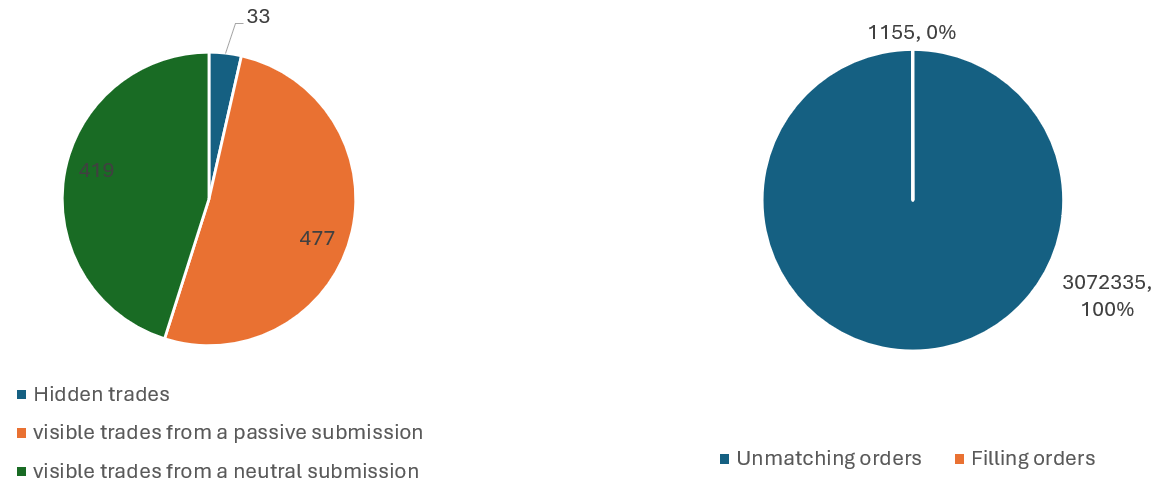
\includegraphics[width=0.8\linewidth]{figures/percentage_of_AT_unmatch.png}
    \caption{Percentage of Passive and Neutral Orders getting filled in the Trade Book and Orders Filled vs. Unmatched in the Order Book}
    \label{fig:p_of_AT_unma}
\end{figure}



\chapter{Methodology}\label{chapter:methodology}
% \setcounter{page}{0}
% \pagenumbering{arabic}
% need change
This chapter discusses mathematical principles of models used in the thesis. The kernel metrics, basic dataset input for training, data processing methods and three prediction models are covered respectively, along with the intuition behind the methodology.

\section{Aggressive Trade}
In the FX trading market, traders may aggressively participate and take out orders which are waiting in the order book. This happens when traders are eager to get trades done, putting more priority in time than price. Once two orders get matched, the information is clearly recorded in trade book data, including the filling price, volume and direction where the order triggers. Normally the filling price for this kind of trade is higher than the best bid/ask price when the aggressive trader intends to submit an order. In contrast to this aggressive trade, it is also common that a trader just put forward a limit order and let it queue in the order flow. After positive market movements, the best bid/ask price matches the order price, the order is likely to get filled if it has the top priority. If the orders are matched, this information is also recorded in the trade book, but with a filling price at the best bid/ask. If it fails to match, it continues to stay in the order book and deepen the order book flow. Besides these two active trading situations, there are plenty of orders silently being submitted or staying and can not find any corresponding records in the trade book at the same timestamp. 

Two targets are provided in Section~\ref{sec: alpha} and Section~\ref{sec: aflag} which describe the trader behaviors in different situations. In the first section we introduce a continuous method to better understand the changing logic, while in the second section the real modeled target is shown and explained.

\subsection{Aggressiveness} \label{sec: alpha}
How aggressive a trader wants to submit orders and match existing orders is worth to discuss in this research. In order to quantify and measure the level, we introduce a metric called \textit{aggressiveness}, denoted by $\alpha$:

\begin{equation}
    \alpha = \frac{P_F - P_B}{P_B}
    \label{eq: aggressiveness}
\end{equation}

$\alpha$ measures the aggressiveness of each trade. $P_F$ is the filling price at the time of the trade, and $P_B$ is the reference price used to determine whether a trade is aggressive. In this context, we set the benchmark as the previous midprice in the order book, i.e., the midprice from the most recent update before the current trade. For example, if a trader wants to buy and places an order above the midprice to grab existing ask orders, this behavior is considered aggressive. The comparison is made against the last observed midprice before the trader submitted the order. 

As shown in Equation~\ref{eq: aggressiveness}, for instance, on the bid side, $\alpha$ is positive if the filling price is higher than the benchmark price. This indicates that a trader is willing to buy at a price above the benchmark. Conversely, $\alpha$ is negative if the trader buys at a price below the benchmark. Similarly, on the ask side, $\alpha$ is negative when a trader sells at a price lower than the benchmark, and positive when the selling price exceeds the benchmark. Therefore, an aggressive trade is defined when $\alpha$ is positive on the bid side and negative on the ask side. When there are no trade records, $\alpha$ is assigned a value of 0. The meanings of different $\alpha$ values are summarized in Table.~\ref{tb: alpha_meaning}:
\begin{table}[h] 
    \centering 
    \begin{tabular}{lll} 
        \toprule 
        \textbf{$\alpha$} & \textbf{Meaning} & \textbf{Data Type} \\ 
        \midrule 
        $ > 0$ & Aggressive bid side trades, or passive ask side trades & Float \\
        $ < 0$ & Aggressive ask side trades, or passive bid side trades & Float \\ 
        $ = 0$ & No trades & Float \\  
        \bottomrule 
    \end{tabular} 
    \caption{Interpretation of $\alpha$ in Different Contexts}
    \label{tb: alpha_meaning}
\end{table}

\subsection{Binary Label for Aggressive Trade} \label{sec: aflag}
However, it is important to note that in the backtesting context at MN, we pay little attention to how aggressive a trader is, whether and when an aggressive trade will occur is more critical. Therefore, based on the $\alpha$, a binary target, called aggressiveness flag, denoted as $\bar{\alpha}$, is introduced. The direction of the trade is not considered by $\bar{\alpha}$ because we assume that traders will adjust order direction according to our order submission dynamically. $\bar{\alpha}$ is set to $0$ if no trade takes place or $\alpha$ is positive in ask side and negative in bid side takes at a given timestamp in the order book, and $1$ if $\alpha$ is possible in bid side and negative in ask side. 
\begin{table}[h] 
    \centering 
    \begin{tabular}{lll} 
        \toprule 
        \textbf{$\bar{\alpha}$} & \textbf{Meaning} & \textbf{Data Type} \\ 
        \midrule 
        $ = 1$ & Aggressive trades & Integer \\
        $ = 0$ & Both passive trades and cases where no trade occurred & Integer \\  
        \bottomrule 
    \end{tabular} 
    \caption{Interpretation of $\bar{\alpha}$ in Different Contexts}
    \label{tb: aflag_meaning}
\end{table}
In Table.~\ref{tb: aflag_meaning}, we get binary flag $\bar{\alpha}$ which contains $1$ and $0$. It is reduced to a classification problem to solve by models, but the complexity of this issue stems from the class balance and feature dependencies. We will discuss them in the following contents in detail.

\section{Data Processing Methods}
% This part describes the dataset used for machine learning training, and resampling and rescale methods
The original order book data and trade book data (Table~\ref{tb: order book data description} and Table~\ref{tb: trade book data description}) fetched from Snowflake and exchange database are too raw to be modeled. In this section, we proceed to discuss methods that are used in data processing. First we discuss feature engineering. It is the process of transforming raw data into meaningful features that enhance the performance of machine learning models. We get effective features based on the calculation of spread, midprice and volume. Then another standard problem: class imbalance is analyzed.

Specifically, in Section~\ref{sec: training data}, we provide basic dataset for model training, test, estimation and prediction, along with specific formulas for certain features. The theoretical solution for extreme class imbalance is established in Section~\ref{sec: class imbalance}.

\subsection{Feature Engineering: Basic Dataset} \label{sec: training data}
In selecting which features to generate, we inherit indicators from original order book and trade book, then extend them to get further features. The target discussed in Section~\ref{sec: aflag} is included as the basic dataset.

\begin{table}[h] 
    \centering 
    \begin{tabular}{lll} 
        \toprule 
        \textbf{Column} & \textbf{Description} & \textbf{Data Type} \\ 
        \midrule 
        $\bar{\alpha}$ & Binary flag & Integer \\
        $T$ & Timestamp of the snapshot in HH:MM.SSS & String \\
        \text{DIRECTION} & Bid($1$) or ask($-1$) trades & Integer \\
        $S$ & Difference between best ask and bid & Float \\
        $M$ & Middle price of best ask and bid & Float\\
        $V_A ^ {1}$ & Volume at best ask & Integer\\
        $V_B ^ {1}$ & Volume at best bid & Integer \\
        %$\alpha$ & How aggressive a trade is & Float \\ 
        %$\tau$ &  &  \\
        $\bar{\delta}_S$ & Average absolute spread change over the past 50 ticks & Float \\
        $\bar{\delta}_M$ & Average absolute mid-price change over the past 50 ticks & Float \\
        $\sigma_S$ & Volatility of spread over the last 50 ticks & Float \\
        $\sigma_M$ & Volatility of mid-price over the last 50 ticks & Float \\
        $r_V$ & Volume imbalance between best ask and bid & Float \\
        \bottomrule 
    \end{tabular} 
    \caption{Overall Dataset for Modeling}
    \label{tb: overall dataset for training}  
\end{table}
In the Table~\ref{tb: overall dataset for training}, capitalized terms refer to variables obtained directly from the order book and trade book data, including timestamp($T$), spread($S$), mid-price($M$), volume($V_A^{1}$, $V_B^{1}$). $T$ represents the time snapshot calculated relative to millisecond.

The last five features ($\bar{\delta}_S$, $\bar{\delta}_M$, $\sigma_S$, $\sigma_M$, $r_V$) are calculated from spread, mid-price or volume based on common factors which display order flow dynamics. $\bar{\delta}_S$ and $\bar{\delta}_M$ measure the local average absolute change over. They both capture the rapid changes in the cost of executing trades, directly related to liquidity changes in real market LOB dynamics. Specifically, $\bar{\delta}_M$ is useful to simulate realistic microstructure scenarios where aggressive trades tend to cluster, such as around price jumps. A 50-tick window is commonly used in high-frequency time series data because it effectively represents the local market environment without unnecessary noise or excessive smoothing. $\bar{\delta}_S$ and $\bar{\delta}_M$ can be formulated as follows:

\begin{equation}
    \bar{\delta}_{S_t} = \frac{1}{50} \sum_{i=0}^{49} \left| S_{t-i} - S_{t-i-1} \right| 
    \label{eq: spread change} 
\end{equation}
\begin{equation}
    \bar{\delta}_{M_t} = \frac{1}{50} \sum_{i=0}^{49} \left| M_{t-i} - M_{t-i-1} \right|
    \label{eq: midprice change} 
\end{equation}

Mid-price realized volatility affects order flows \citep{LO2010213}, thus $\sigma_M$ is used to depict the variability of mid-price changes. As defined in Equation~\ref{eq: midprice vola} and \ref{eq: spread vola}, standard deviation of mid-price changes and spread changes are calculated over a rolling window of 50 ticks. Spread factor $\sigma_S$ is also included because it reflects the consistency and variability of liquidity conditions.

\begin{equation}
    \sigma_{S_t} = \sqrt{\frac{1}{49}\sum_{i=0}^{48}\left((S_{t - i}-S_{t - i - 1})-\bar{\delta}_{S_t}\right)^2}
    \label{eq: spread vola}
\end{equation}

\begin{equation}
    \sigma_{M_t} = \sqrt{\frac{1}{49}\sum_{i=0}^{48}\left((M_{t - i}-M_{t - i - 1})-\bar{\delta}_{M_t}\right)^2}
    \label{eq: midprice vola}
\end{equation}

Higher $\bar{\delta}$ ($\bar{\delta}_S$ and $\bar{\delta}_M$) indicates that the market experiences frequent, sizable changes, with higher $\bar{\delta}_S$ reflecting unstable liquidity, and higher $\bar{\delta}_M$ showing active price discovery and increased market uncertainty. Conversely, lower $\bar{\delta}$ values signify stability, with lower $\bar{\delta}_S$ indicating consistent liquidity, and lower $\bar{\delta}_M$ suggesting calmer, more stable price movements.

Higher $\sigma$ ($\sigma_M$ and $\sigma_S$) represents greater variability and unpredictability in the market, with higher $\sigma_{S}$ highlighting liquidity risk, and higher $\sigma_{M}$ means significant fluctuations and uncertainty in the mid-price. Lower $\sigma$ denotes more predictable conditions, where lower $\sigma_{S}$ indicates stable liquidity conditions and lower $\sigma_{M}$ reflects reduced price uncertainty and market stability.

$r_V$ represents the relative imbalance between the ask and bid sides, as defined in Equation.~\ref{eq: volume ratio}. When $r_V$ approaches 1, most of the volume is concentrated on the ask side, indicating selling pressure in the limit order book. Conversely, when it approaches $-1$, the volume is mainly on the bid side, suggesting buying pressure. If $r_V$ is close to 0, the volumes are approximately balanced.
\begin{equation}
    r_V = \frac{V_A ^ {1} - V_B ^ {1}}{V_A ^ {1} + V_B ^ {1}}
    \label{eq: volume ratio}
\end{equation}


\subsection{Extreme Class Imbalance Solution} \label{sec: class imbalance}
% What is class imbalance
In a binary classification problem with data samples from two groups, class imbalance occurs when one class, the minority group, contains significantly fewer samples than the other class, the majority group \citep{johnson_survey_2019}. Extreme class imbalance refers to scenarios where the minority class represents less than 1\% of the total dataset \citep{leevy_survey_2018}. This level of imbalance brings significant challenges for machine learning algorithms, with strong bias results toward the majority class and may completely ignore the minority class in extreme cases. Extremely imbalanced datasets like this one are common in medicine and finance fields.

To predict aggressive trades in the limit order book, we study the aggressive trade flag ($\bar{\alpha}$). To demonstrate the imbalance clearly, one of a trading day is selected here, as shown in Figure.~\ref{fig: aflag_class_distribution}. $\bar{\alpha}$ faces severe class imbalance, which can lead to biased model predictions if not addressed. In the figure, class 0 dominates the dataset, accounting for 99.8\% of all samples, while Class 1 accounts for only 0.2\%. To solve this imbalance, techniques such as resampling, weighted loss function, and anomaly filter function are employed. 
\begin{figure}[h]
    \centering
    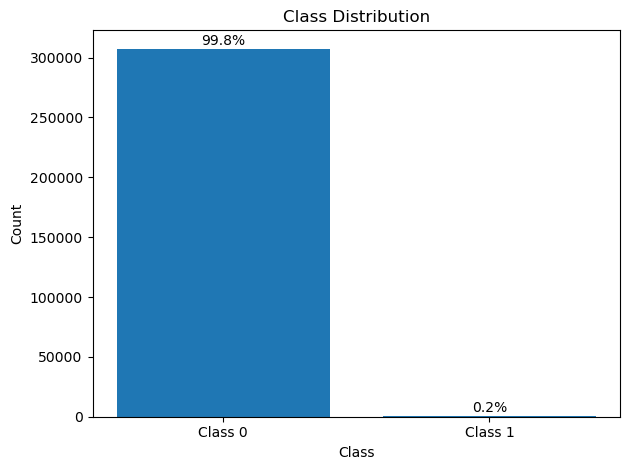
\includegraphics[width=0.8\linewidth]{figures/Imbalaced data for aflag.png}
    \caption{Class Distribution for $\bar{\alpha}$ on 31st January. In the overall 308,178 data, class 0 accounts for 99.8\% of the samples, while Class 1 represents only 0.2\%, indicating a severe class imbalance.}
    \label{fig: aflag_class_distribution}
\end{figure}

SMOTE (Synthetic Minority Over-sampling Technique) is an advanced oversampling method that generates synthetic samples of the minority class by interpolating between existing ones. However, since SMOTE connects both inliers and outliers arbitrarily, it may lead to a sub-optimal decision boundary, especially in high-dimensional and noisy datasets of our case. To better fit our dataset, we adopt a SMOTE variant called KMeansSMOTE, which applies KMeans clustering before performing oversampling. This clustering step groups similar samples together and generates synthetic data based on cluster density. For our high-frequency and extremely imbalanced data, KMeansSMOTE helps prevent synthetic samples from being generated in sparse or noisy regions, and creates more informative minority class samples that reflect the local data structure.
Let $\mathcal{X}_{\text{min}} = \{x_1, \dots, x_{N_{\text{min}}}\} \subset \mathbb{R}^d$ be the minority class. KMeansSMOTE proceeds as follows:

Apply KMeans to $\mathcal{X}_{\text{min}}$ with $k$ clusters:
  \[
  \min_{\{C_j\}} \sum_{j=1}^k \sum_{x \in C_j} \|x - \mu_j\|^2, \quad \mu_j = \frac{1}{|C_j|} \sum_{x \in C_j} x
  \]

For each cluster $C_j$, compute:
  \[
  \text{Density}_j = \frac{|C_j|}{\text{avg\_intra\_dist}(C_j)}, \quad w_j = \frac{1/\text{Density}_j}{\sum_{i} 1/\text{Density}_i}
  \]
where avg\_intra\_dist is the average pairwise distance within $C_j$. Set $n_j = \lfloor w_j \cdot n_{\text{gen}} \rfloor$.

For each $C_j$, repeat $n_j$ times:
  \[
  \tilde{x} = x + \lambda (x^{\text{NN}} - x), \quad \lambda \sim \mathcal{U}(0, 1)
  \]
where $x, x^{\text{NN}} \in C_j$ are randomly selected minority points and one of its $k$ nearest neighbors.

Building upon the foundation laid in the balanced class, weighted loss functions are implemented during the machine learning training process to focus on the accuracy of class 1. For example, in XGBoost, the weight is applied to the loss function by assigning a higher importance to the misclassification of class 1 samples. Specifically, the objective function includes a weighted logistic loss where the weight $w_i$ for each instance increases if the sample belongs to the target class, influencing both the gradient and Hessian in the boosting process. Additionally, take GRU-based RNN for another example, class weights are introduced in the binary cross-entropy loss function. The loss becomes:
\[
\mathcal{L} = -w_1 \cdot y \cdot \log(\hat{y}) - w_0 \cdot (1 - y) \cdot \log(1 - \hat{y})
\]
where $w_1$ and $w_0$ are the weights for class 1 and class 0, respectively, $y$ is the true label, and $\hat{y}$ is the predicted probability. This weighted loss penalizes the model more for errors on class 1, guiding it to pay more attention to the target class during training.

Anomaly filter methods are also applied to highlight the regions around aggressive trading events. This thesis presents a window-based filter function to extract time segments centered around class 1 instances. Specifically, for each sample with a non-missing DIRECTION label, which means there is at least one trade recorded, a window of certain milliseconds is defined. All entries within this time range are included for training. This method ensures that the model is exposed to a richer context around potential anomalies and enhances the learning of class 1 patterns in the high-frequency setting. In our practical implementation, we integrate an anomaly detection function alongside KMeansSMOTE across different models. This ensures that imbalanced class problem are handled without conflict in each model and maintains balanced class distributions consistently between the models.

\begin{algorithm}[H]
\caption{Window-Based Anomaly Filter} \label{al: window-based}
\begin{algorithmic}[1]
\State \textbf{Input:} Data with timestamps and labels; window size $\delta$
\State \textbf{Output:} Filtered data around class 1 instances
\For{each timestamp $t$ where \texttt{DIRECTION} is not NaN}
    \State Define window: $[t - \delta/2,\ t + \delta/2]$
    \State Find all rows within this window and add their indices to \texttt{result\_indices}
\EndFor
\State \Return rows corresponding to \texttt{result\_indices}
\end{algorithmic}
\end{algorithm}


\section{Prediction Model: An XGBoost-Enhanced Neural Hawkes Process Framework}
This thesis proposes an XGBoost-enhanced Neural Hawkes Process framework combining class imbalance solutions, neural encoder, and stochastic modeling to predict aggressive trades under extreme class imbalance. The framework is designed to first resolve class imbalance through resampling in XGBoost, then integrate nonlinear and long-range feature dependencies, which are extracted from recurrent neural networks, into the calculation of intensity in Hawkes processes. 

The framework begins with an XGBoost classifier trained to identify aggressive trade events from limit order book features displayed in Table~\ref{tb: overall dataset for training}. To address the extreme class imbalance in the dataset, KMeansSMOTE is applied during training to generate synthetic minority samples in a structure-aware manner, ensuring a more balanced and representative training set. The first-filtered output of the XGBoost model, alongside features, is then fed into a Gated Recurrent Unit (GRU), which acts as a historical market state encoder. The GRU transforms the inputs into a compact hidden state that captures nonlinear dependencies and long-range dynamics in condition of temporal logic ($T$) and market features ($S$, $M$, $V_A^{1}$, $V_A^{1}$, $\bar{\delta}_S$, $\bar{\delta}_M$, $\sigma_S$, $\sigma_M$, $r_V$). This hidden state is used to condition the intensity function $\lambda(t)$ of a neural Hawkes process. Unlike classical Hawkes models based on additive exponential kernels, the intensity here is dynamically modulated by the GRU output, allowing the model to flexibly capture evolving market microstructure behavior. As a result, the process becomes a conditional point process, where the estimation of parameters is informed by both structured and balanced output of the XGBoost model and the latent dynamics embedded in recent order book activity.

In the first stage, we employ XGBoost to predict $\bar{\alpha}$ on the full trading day using limit order book features in Table~\ref{tb: overall dataset for training}. To address the extreme class imbalance and get potential aggressive trade rows, we apply KMeansSMOTE before training. This first classifier aims to identify as many true trade points as possible (high recall) and increase the proportion of minor class in the output. The model filters out most of the non-aggressive instances (class 0) and provides a broad set of aggressive trade activity candidates. This output serves two purposes: it reduces the candidate space for aggressive trade prediction, and its feature importance guides the selection of input features for subsequent models.

In the second stage, we train a GRU-based recurrent neural network to get the hidden state formula of the two market scenarios as mentioned in Table~\ref{tb: aflag_meaning} (aggressive and non-aggressive). The GRU model is trained on a balanced dataset constructed using a window-based anomaly filter function around class 1 labels as presented in Algorithm~\ref{al: window-based}. This stage further refines the prediction of aggressive trades by deep learning networks. The GRU hidden state captures these invisible market conditions that traditional Hawkes can not see, but that critically affect event intensity.

In the final stage, we apply a neural Hawkes process to analyze a more dynamic estimation and prediction of aggressive trades. The Hawkes model captures the temporal clustering of aggressive trade events and demonstrates interpretable output in the form of aggressive and non-aggressive trade intensity and probability. This significantly compensates for the limited ability of machine learning models. We also incorporate a condition based on MN trade execution information: if an internal order is filled within certain milliseconds window, it increases the likelihood of a nearby aggressive trade. This step not only enhances the final accuracy and F1 score, but also produces a more interpretable, precise and inclusive prediction set.

Overall, this three-stage framework effectively predicts rare aggressive trades by combining class imbalance solution, market states features, sequential memory, and temporal dependency modeling. It predicts the intensity and final pattern of aggressive and non-aggressive events. The following parts of the section elaborate each of the three components and discuss the combined contribution of the predictive framework.

\subsection{XGBoost with KMeansSMOTE Filtering (KM-XGBoost)}
XGBoost is a tree-based ensemble learning method that builds a sequence of decision trees to minimize a specified loss function. With a gradient boosting logic, each new tree is trained on the residual errors of the current model, effectively correcting its mistakes by following the negative gradient of the loss. 

XGBoost is a strong overall model, which includes features that make it especially practical and powerful in real-world applications. \cite{XGBoost_2016} compare XGBoost with some other popular classifiers, and find XGBoost helps prevent overfitting through built-in regularization, can handle sparse data automatically without preprocessing, and is optimized for speed and memory efficiency, making it well-suited for large-scale datasets with imbalanced data. XGBoost can capture nonlinear patterns that logistic regression cannot, and handles sparse data with native sparsity-aware algorithms. Compared to GBM (Traditional Gradient Boosting Machines), XGBoost significantly outperforms them in training time (up to 10x faster) and often in test accuracy. In the context of Kaggle competitions, XGBoost outperforms neural networks, especially in tabular data, and top entries use XGBoost rather than deep learning models \citep{XGBoost_2016}. It represents that XGBoost is easier to tune and more robust to hyperparameter choices in those settings and less data-hungry than deep neural nets.

The underlying objective function of XGBoost can be explained as follows: a loss term and a regularization term. It is defined as:

\begin{equation}
\mathcal{L}(\phi) = \sum_{i=1}^{n} l(y_i, \hat{y}_i^{(t)}) + \sum_{k=1}^{t} \Omega(f_k)
\end{equation}

Where $l$ is a differentiable convex loss function, such as the logistic loss for binary classification. It measures the difference between the true label $y_i$ and the predicted value $\hat{y}_i^{(t)}$ at iteration $t$. The second term, $\Omega(f_k)$, is a regularization function that penalizes the complexity of each added tree $f_k$.

The regularization term is defined as:

\begin{equation}
\Omega(f) = \gamma T + \frac{1}{2} \lambda \|w\|^2
\end{equation}

Here, $T$ denotes the number of leaves in the regression tree, $w$ represents the vector of scores assigned to the leaves, and $\gamma$, $\lambda$ are regularization parameters that control the penalty on the number of leaves and the magnitude of leaf weights respectively. If $T$ is larger, it gives better data fitting and gets penalties by $\lambda$ and $\lambda \|w\|^2$, avoiding overfitting.

This thesis uses GridSearchCV and cross-validation to find the best hyperparameters for the XGBoost model. GridSearchCV is a module from the Python library scikit-learn \citep{scikit-learn2011}, which performs an ergodic search over a grid of hyperparameter values. It combines this with cross-validation, a technique that splits the training data into multiple folds. In each round, one fold is used for validation and the others for training. This helps to evaluate the model performance more fairly and avoids overfitting to one specific subset of data. 

Algorithm~\ref{alg: grid_search} demonstrates the setup of hyperparameter tuning. The search is conducted over three values each for $n\_estimators$ (number of boosting rounds), $max\_depth$, $learning\_rate$, and $min\_child\_weight$. One fixed value of $scale\_pos\_weight$, which was computed based on the class imbalance ratio. The evaluation metric used is ROC-AUC, which is especially suitable for imbalanced classification tasks. A 3-fold cross-validation ($cv=3$) is applied, and the search is performed in parallel using all available CPU cores ($n\_jobs=-1$) for efficiency. To give more focus on aggressive trades, instance weights are manually adjusted before fitting: class 1 (aggressive trades) is assigned a higher weight (100.0), while class 0 (non-aggressive trades) receives a weight of 1. This weighting helps the model pay more attention to aggressive trades during training.

% \begin{algorithm}[H]
% \caption{Grid Search with Cross-Validation for XGBoost} \label{alg: grid_search}
% \begin{algorithmic}[1]
%     \State Define base XGBoost model with fixed settings:
%     \Statex \hspace{\algorithmicindent} \texttt{use\_label\_encoder=False}, \texttt{eval\_metric='logloss'}, \texttt{random\_state=42}
%     \State Define hyperparameter grid:
%     \Statex \hspace{\algorithmicindent} \texttt{n\_estimators} $\in \{100, 300, 500\}$
%     \Statex \hspace{\algorithmicindent} \texttt{max\_depth} $\in \{3, 5, 7\}$
%     \Statex \hspace{\algorithmicindent} \texttt{learning\_rate} $\in \{0.01, 0.02, 0.05\}$
%     \Statex \hspace{\algorithmicindent} \texttt{min\_child\_weight} $\in \{3, 5, 7\}$
%     \Statex \hspace{\algorithmicindent} \texttt{scale\_pos\_weight} = computed class imbalance ratio
%     \State Initialize GridSearchCV with:
%     \Statex \hspace{\algorithmicindent} scoring metric: ROC-AUC
%     \Statex \hspace{\algorithmicindent} cross-validation folds: 3
%     \Statex \hspace{\algorithmicindent} parallel jobs: all CPUs (\texttt{n\_jobs=-1})
%     \State Compute sample weights:
%     \Statex \hspace{\algorithmicindent} weight = 100.0 for aggressive trades
%     \Statex \hspace{\algorithmicindent} weight = 1.0 for non-aggressive trades
%     \State Fit model to resampled training data using \texttt{sample\_weight}
%     \State Return best hyperparameters and cross-validated model
% \end{algorithmic}
% \end{algorithm}

\begin{algorithm}[H]
\caption{Grid Search with Cross-Validation for XGBoost}\label{alg: grid_search}
\begin{algorithmic}[1]
    \State Define base XGBoost model:
    \Statex \hspace{\algorithmicindent} \texttt{use\_label\_encoder=False}, \texttt{eval\_metric='logloss'}, \texttt{random\_state=42}
    \State Define base XGBoost model with fixed settings:
    \Statex \hspace{\algorithmicindent} \texttt{use\_label\_encoder=False}, \texttt{eval\_metric='logloss'}, \texttt{random\_state=42}
    \State Define hyperparameter grid:
    \Statex \hspace{\algorithmicindent} \texttt{n\_estimators} $\in \{100, 300, 500\}$
    \Statex \hspace{\algorithmicindent} \texttt{max\_depth} $\in \{3, 5, 7\}$
    \Statex \hspace{\algorithmicindent} \texttt{learning\_rate} $\in \{0.01, 0.02, 0.05\}$
    \Statex \hspace{\algorithmicindent} \texttt{min\_child\_weight} $\in \{3, 5, 7\}$
    \Statex \hspace{\algorithmicindent} \texttt{scale\_pos\_weight} = computed class imbalance ratio
    \State Initialize GridSearchCV with:
    \Statex \hspace{\algorithmicindent} scoring metric: ROC-AUC
    \Statex \hspace{\algorithmicindent} parallel jobs: all CPUs (\texttt{n\_jobs=-1})
    \State Compute sample weights:
    \Statex \hspace{\algorithmicindent} weight = 100.0 for aggressive trades
    \Statex \hspace{\algorithmicindent} weight = 1.0 for non-aggressive trades
    \ForAll {hyperparameter combinations in grid}
        \For{fold $k = 1$ to $K$ (e.g. 3)}
            \State Split data into training set $D_{\text{train}}^{(k)}$ and validation set $D_{\text{val}}^{(k)}$
            \State Train model on $D_{\text{train}}^{(k)}$ using sample weights
            \State Evaluate ROC-AUC on $D_{\text{val}}^{(k)}$
        \EndFor
        \State Compute average ROC-AUC across $K$ folds
    \EndFor
    \State Select the hyperparameter set with the highest average ROC-AUC
    \State Re-train final model on full training set using selected hyperparameters
\end{algorithmic}
\end{algorithm}

The architecture of XGBoost encourages the model to fit the data effectively with awareness of class focus, while avoiding overfitting by controlling model complexity. This results in a faster and more practical training process.

In our study, KMeansSMOTE is applied to the training data to address class imbalance before feeding it into XGBoost. XGBoost is then used to predict $\bar{\alpha}$ and to generate feature importance scores. These scores serve as a reference for selecting relevant features in the subsequent neural network training. This feature selection step helps reduce model complexity and focuses the learning process on the most informative patterns. The input-output workflow of this process can be summarized as follows:
\begin{itemize}
  \item \textbf{Input:}  
  The model receives a resampled dataset obtained by applying KMeansSMOTE to the original data presented in Table~\ref{tb: overall dataset for training}. The resampling adjusts the class distribution to approximately 3:7 (aggressive:non-aggressive). Input features include engineered features $S$, $M$, $V_A^{1}$, $V_A^{1}$, $\bar{\delta}_S$, $\bar{\delta}_M$, $\sigma_S$, $\sigma_M$, $r_V$.

  \item \textbf{Model Configuration:}  
  An XGBoost classifier is trained using hyperparameters selected via GridSearchCV. The final model configuration is:
  \begin{itemize}
    \item \texttt{n\_estimators} = 500
    \item \texttt{max\_depth} = 7
    \item \texttt{min\_child\_weight} = 5
    \item \texttt{learning\_rate} = 0.05
    \item \texttt{scale\_pos\_weight} = computed imbalance ratio
    \item \texttt{eval\_metric} = 'logloss'
    %\item \texttt{random\_state} = 42
  \end{itemize}

  \item \textbf{Output:}  
  The model outputs a binary prediction for each record in the time window of a given trading day, indicating whether the event is likely to be an aggressive trade (\texttt{class = 1}). The output gives a more balanced class dataset, with the class 1 (aggressive trade) accounting for approximately 10\% of the whole data.

\end{itemize}

\begin{figure}[H]
\centering
\begin{tikzpicture}[node distance=2cm]

\node (data) [block] {Original Training Data \\ (Table~\ref{tb: overall dataset for training})};
\node (resample) [block, below of=data] {KMeansSMOTE \\ (Class ratio 3:7)};
\node (xgboost) [block, below of=resample] {XGBoost Classifier \\ (Tuned via GridSearchCV)};
\node (output) [block, below of=xgboost] {Predicted Class \\ (Aggressive Trade ~10\%)};

\draw [arrow] (data) -- (resample);
\draw [arrow] (resample) -- (xgboost);
\draw [arrow] (xgboost) -- (output);

\end{tikzpicture}
\caption{XGBoost input-output workflow for aggressive trade prediction.}
\label{fig:xgboost-flow}
\end{figure}

%-------------------------GRU-----------------------------
\subsection{Gated Recurrent Units (GRU)-based RNN}
% what's GRU
To model the nonlinear and long-range sequential dynamics in condition of market features of aggressive trades, we employ a recurrent neural network (RNN) based on GRU. GRU is a type of neural network designed to work with sequential data alongside engineered features, such as time series, sentences, or trading records. Unlike standard models that treat each input independently, a GRU learns from past information and current input at the same time. When we deal with data that unfolds over time, like a series of trades, it's important to understand how earlier events influence later ones. For example, an aggressive trade might be more likely to happen now if the spread was very low several ticks ago. 

% why GRU not others
GRU is a simplified variant of the Long Short-Term Memory (LSTM) network, designed to capture long-range dependencies while using fewer parameters and computational resources \citep{GRU2014}. It has a simplified architecture with two gates: the update gate and reset gate. The update gate controls how much of the previous hidden state should be retained, and the reset gate determines how much of the past information to forget. The two gates allow the model to remember or forget past information as needed, crucial for understanding market patterns in order book data. Since it lacks the forget gate, compared to LSTM, GRU has fewer parameters and faster training times, making it more efficient for larger datasets. In many cases, the performance difference between LSTM and GRU is not significant, and GRU is often preferred due to its simplicity and efficiency. 

In our study, we adopt a GRU architecture instead of the LSTM structure used by \cite{lalor2025eventbasedlimitorderbook} because our problem involves fewer event types, but much higher frequent dynamics, where fast and robust convergence is critical. More specifically, Table~\ref{tab:gru_vs_lstm} compares the use of GRU with the LSTM approach used by \cite{lalor2025eventbasedlimitorderbook}.

\begin{table}[H]
\centering
\caption{Comparison of LSTM-Based Model vs. GRU-Based Model}
\begin{tabular}{p{3cm} p{5.5cm} p{5.5cm}}
\toprule
\textbf{Aspect} & \textbf{LSTM-Based Model} & \textbf{GRU-Based Model} \\
\midrule
\textbf{Data Domain} & Stock LOBSTER data (lower tick frequency, long time span) & FX spot market data (millisecond frequency, short time window) \\
\textbf{Purpose} & Simulates all 12 LOB event types & Predicts binary outcome \\
\textbf{Complexity} & High: expressive but computationally intensive & Low: efficient and sufficient for task-specific modeling \\
\textbf{Training Time} & Slower convergence; more resource intensive & Faster training; lightweight structure \\
\textbf{Overfitting Risk} & High: due to model size and variable performance across assets & Lower: binary setting with consistent performance \\
\bottomrule
\end{tabular}
\label{tab:gru_vs_lstm}
\end{table}

On the one hand, the LSTM-based approach is designed to handle a large and diverse set of 12 LOB event types. This level of event complexity and inter-type interaction needs a more complicated but also heavier architecture like LSTM. In contrast, our setting focuses on a simpler and more specific prediction task. Our training dataset contains just two types of market scenarios (aggressive vs. non-aggressive trades). We do not simulate all LOB events but instead focus on binary classification. Therefore, the computational burden of LSTM is unnecessary, and the more efficient GRU offers a faster and equally expressive alternative for our goal.

On the other hand, \cite{lalor2025eventbasedlimitorderbook} rely on stock data from LOBSTER. It is relatively lower tick frequencies compared to higher-frequent FX spot markets. As a result, fast and robust convergence is critical. GRU is a more suitable RNN to predict aggressive trade pattern in the high frequency FX spot market.


% why hidden states matter and math formulas
GRU helps the model remember those earlier patterns by giving a hidden state. It is a memory storage that is updated at each step in the sequence. The core assumption behind using an RNN is that the current output depends not only on the current input but also on the historical sequence of past inputs. Formally, a GRU updates its hidden state through gating mechanisms that regulate the flow of information, allowing it to selectively retain or forget past information as needed. It can consist of multiple stacked GRU layers and be followed by a dense output layer. Each GRU layer returns sequences to preserve the full temporal structure across time steps. The model is trained to minimize a weighted mean squared error (MSE) loss. 
\begin{equation}
    \mathcal{L} = \frac{1}{N} \sum_{i=1}^{N} \sum_{t=\text{warmup\_steps}}^{T} w_{i,t} \left( y_{i,t} - \hat{y}_{i,t} \right)^2
    \label{eq:GRU loss function}
\end{equation}
    where
\begin{equation}
    w_{i,t} =
    \begin{cases}
    w_\text{nozero}, & \text{if } y_{i,t} \neq 0 \\
    w_\text{zero}, & \text{if } y_{i,t} = 0
    \end{cases}
    \label{eq:weight in GRU loss}
\end{equation}
    
In Equation.~\ref{eq:GRU loss function} and \ref{eq:weight in GRU loss}, higher importance is given to nonzero targets to emphasize the prediction of aggressive behaviors. Furthermore, the initial warmup steps are ignored in each sequence when calculating the loss. During this phase, hidden state representations are still developing, and their predictions are often noisy \citep{lambrechts2023warmingrecurrentneuralnetworks}. This can prevent the model from being penalized during its early and uncertain predictions.

The GRU works through four simple steps. First, the reset gate $r_t$ decides how much of the previous memory to forget when creating new information. If values close to 0, it forgets most of the past and values, while values closing to 1 mean remember everything. Next, the update gate $z_t$ acts as a mixing controller that determines how much to blend old memory with new information. The candidate hidden state $\tilde{h}_t$ represents the proposed new memory based on the current input. Finally, the most important part, actual hidden state $h_t$, is computed as a weighted average between the old memory and the new candidate. It controls how much of the old memory should be used to create new information, and how much should the memory be updated with this new information.
\begin{align}
    % Reset Gate
    r_t = \sigma(W_r \cdot [h_{t-1}, x_t] + b_r) \\
    % Update Gate
    z_t = \sigma(W_z \cdot [h_{t-1}, x_t] + b_z) \\
    % Candidate Hidden State
    \tilde{h}_t = \tanh(W_h \cdot [r_t \odot h_{t-1}, x_t] + b_h) \\
    % Final Hidden State
    h_t = (1 - z_t) \odot h_{t-1} + z_t \odot \tilde{h}_t
\end{align}

% input and output
In our study, the model is trained to capture hidden states which can keep useful memory of past inputs. These hidden states are later used as dynamic inputs for the Hawkes process. It works well enough for our binary trade prediction task and helps connect market features with intensity estimation. The input-output workflow of this process can be summarized as follows:

\begin{itemize}
  \item \textbf{Input:}  
  An anomaly filter is applied to the raw dataset. For each record with a valid \texttt{DIRECTION} label, a fixed-width time window is constructed. All entries falling within this window are collected to form a training sample. This ensures the filtered dataset maintains approximately 10\% aggressive trades, aligning with the XGBoost classifier's output distribution.

  Before training, features (\texttt{x\_train}) and labels (\texttt{y\_train}) are scaled using \texttt{MinMaxScaler()}, and sequences are reshaped with a fixed length of 3000 time steps. The training is conducted using a batch size of 32.

  \item \textbf{Model Configuration:}  
  A GRU-based model is defined using Keras \texttt{Sequential()}:
  \begin{itemize}
    \item First layer: GRU with 1024 units, returning sequences.
    \item Second layer: Fully connected \texttt{Dense} layer with sigmoid activation.
    \item Optimizer: RMSprop with learning rate $10^{-3}$
    \item Loss function: custom \texttt{loss\_mse\_warmup} to exclude initial warmup steps from the loss.
  \end{itemize}

  The model is trained with \texttt{model.fit()} using a generator that yields sequences, over 6 epochs with 6 steps per epoch. These settings are selected based on convergence behavior.

  \item \textbf{Output:}  
  After training, a hidden state extraction function is applied to retrieve the dynamic GRU hidden states at each timestamp for both aggressive (class 1) and non-aggressive (class 0) trades. These hidden states are then used to condition the intensity function in the subsequent Hawkes process.
\end{itemize}

\begin{figure}[H]
\centering
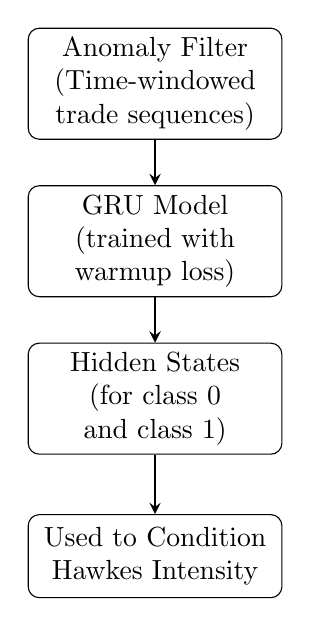
\begin{tikzpicture}[node distance=2cm]

    \tikzstyle{block} = [rectangle, draw, text width=8.5em, align=center, rounded corners, minimum height=3em]
    \tikzstyle{arrow} = [thick,->,>=stealth]

    \node (filtered) [block] {Anomaly Filter\\ (Time-windowed trade sequences)};
 
    \node (gru) [block, below of=filtered] {GRU Model\\ (trained with warmup loss)};

    \node (hidden) [block, below of=gru] {Hidden States\\ (for class 0 and class 1)};

    \node (hawkes) [block, below of=hidden] {Used to Condition\\ Hawkes Intensity};

    \draw [arrow] (filtered) -- (gru);
    \draw [arrow] (gru) -- (hidden);
    \draw [arrow] (hidden) -- (hawkes);

\end{tikzpicture}
\caption{Input-output flow of the GRU-based encoder.}
\label{fig:gru-flow}
\end{figure}


\subsection{Neural Hawkes Process}
% what is Hawkes and how our neural HP nice
The Hawkes process is a self-exciting point process that models events happening over time. It is called 'self-exciting' because each event can make future events more likely (or less likely) to happen soon after. This is different from normal classification models that give a yes-or-no answer. The Hawkes process gives a time-varying intensity function, written as $\lambda(t)$, which represents the conditional probability density of the occurrence of an event in the immediate future \citep{bacry2015hawkesprocessesfinance}. 

We use a neural Hawkes process to improve this traditional model. Instead of using fixed formulas, we let a neural network reinforce the calculation of the intensity function. This makes the model more flexible and able to fit complex patterns, like how the memory of past trades changes over time and how the historical market features affect current situations. By the way of GRU learning hidden patterns in the order book sequence, using its hidden states inside the Hawkes model allows us to connect trading signals with time-based predictions in a natural way. This design is especially useful for modeling latent, event-driven and clustering data like trades in the FX market.


% why integrate hidden states instead of traditional HP
By formulating a neural kernel from GRU-based RNNs, the model extends traditional Hawkes process which uses a fixed parametric form for the intensity function. The idea of predicting aggressive trades based on the structure of a GRU-Hawkes process is new and novel.


% how hidden states and trade aware are used in math formula
A key innovation in our approach is the hidden state integration and trade-aware intensity adjustment. We multiple the GRU hidden state $h_t$ to initial intensity formula. This helps capture these invisible market conditions that traditional Hawkes cannot see but that critically affect event intensity. Moreover, we add an additional term to the intensity function: if one of our own trades occurs within certain milliseconds of a candidate time $t$, we increase the intensity $\lambda(t)$ by a small boost $\delta$. This reflects the idea that our own trading activity may affect the likelihood of surrounding market behavior. The adjusted conditional intensity function is given by:

\begin{equation}
\lambda_k(t) = (\mu_k + \sum_{j=1}^{K} \sum_{t_i^j < t} \alpha_{kj} e^{-\beta_{kj}(t - t_i^j)}) \times \log(1+e^{h_k(t)}) + \delta \cdot \mathbf{1}_{\{\exists \tau \in \mathcal{T}_{\text{own}},\ |t - \tau| \leq \Delta \}}
\end{equation}

Where $\mu_k$ is the baseline intensity, $\alpha$ controls excitation (how much one event influences others), $\beta$ is the decay rate, $t_i^j$ are past event times. $h_k(t)$ is the hidden states from GRU. The last term adds influence from our own trades.

Once the intensity function is fitted, we simulate predicted aggressive trade times using Ogata's thinning algorithm. This method samples from a Poisson process with an upper-bound rate, then accepts each sample with probability proportional to the true intensity $\lambda(t)$.

% how I use it
We represent trade types using a one-hot encoded vector:
Due to the high computational cost of fitting Hawkes models on large-scale data, we only apply it to the filtered, lightweight dataset produced by GRU anomaly filter. This improves feasibility, reduces noise, and keeps precision.
\begin{center}
\begin{tabular}{lll}
(1, 0) & : & No trade or Passive trade \\
(0, 1) & : & Aggressive trade \\
\end{tabular}
\end{center}
This clearly distinguishes trading behavior at each timestamp. The passive trades are combined with no-trade events because they are not our prediction target.

% why it's more interpreable
This modeling approach allows us to preserve more realistic and interpretable signals for aggressive trade detection. Higher intensity in the aggressive trade dimension implies higher probability of retaining that point as a simulated aggressive trade. It complements the previous stages by capturing both temporal clustering and the effect of our own executions.


\section{Whole Framework}


\section{Evaluation Metrics}

\subsection{Data Performance}
% filter ratio, Class Distribution

\subsection{Confusion Matrix}
% TP, TN, FP, FN

\subsection{Classification Report}
% Precision, recall, F1-score, Relaxed Metrics






% \subsection{Two-stage Generative Adversarial Network}
% To generate realistic synthetic time series, we adopt a two-stage generative adversarial network (GAN). The model consists of two interconnected components: the first WGAN, denoted as \( G_1 \), maps random latent vectors \( z \sim \mathcal{N}(0, I) \) into synthetic spectrogram images \( G_1(z) \), capturing the global frequency-domain structure. The second conditional WGAN, denoted as \( G_2 \), takes these spectrograms as input and generates corresponding time series \( G_2(G_1(z)) \). Both stages are trained by minimizing the Wasserstein loss with gradient penalty:

% \begin{equation}
% \mathcal{L}_{\text{WGAN-GP}} = \mathbb{E}_{x \sim P_r}[D(x)] - \mathbb{E}_{\tilde{x} \sim P_g}[D(\tilde{x})] + \lambda \mathbb{E}_{\hat{x} \sim P_{\hat{x}}}\left[\left(\|\nabla_{\hat{x}} D(\hat{x})\|_2 - 1\right)^2\right],
% \end{equation}

% where \( D \) is the critic, \( P_r \) is the real data distribution, \( P_g \) is the generated data distribution, and \( P_{\hat{x}} \) is the distribution of interpolated samples. The use of spectrograms as intermediate representations enables the first generator to capture rich latent patterns over multiple time scales, while the second generator focuses on reconstructing realistic temporal dynamics.

% It's useful when data has complex multi-scale patterns and very little data (few-shot).


% \subsection{Time-Conditional Generative Adversarial Network}
% The Time-Conditional Generative Adversarial Network (T-CGAN) consists of a generator \( G \) and a discriminator \( D \), both conditioned explicitly on timestamp sequences. Given a noise vector \( z \sim p_z(z) \) and a timestamp vector \( t \sim p_T(t) \), the generator \( G(z|t) \) produces synthetic time series aligned with the conditional timestamps, while the discriminator \( D(x|t) \) evaluates whether a given time series \( x \) conditioned on \( t \) is real or generated. The training objective follows a conditional GAN formulation:

% \begin{equation}
% \min_{G} \max_{D} V(D,G) = \mathbb{E}_{x \sim p_{\text{data}}(x)} \left[\log D(x|t)\right] + \mathbb{E}_{z \sim p_z(z)} \left[\log(1 - D(G(z|t)))\right],
% \end{equation}

% where \( p_{\text{data}}(x) \) represents the real data distribution. The generator is implemented as a convolutional neural network (CNN) with deconvolution layers, while the discriminator uses convolutional layers with max pooling. By conditioning both the generator and discriminator on timestamps, T-CGAN learns the relationship between temporal irregularities and data values, allowing realistic augmentation of short, noisy, and unevenly sampled sequences. This design is particularly suited for scenarios where irregular sampling and small data availability hinder traditional time series modeling approaches.

% It's useful when we want to preserve sampling irregularity in generated data.


\chapter{Empirical Experiments}\label{chapter:experiments}
% \setcounter{page}{0}
% \pagenumbering{arabic}

\section{Prices and Filling Information}
To have a comprehensive understanding of how trades in trade book correspond to orders in order book, Figure~\ref{fig:p_f_i} provides an overview of the whole active trading hours from 10:00 am to 4:00 pm on 31st January. It shows how filled price in the trade book track the mid-price in the order book, the distribution of passive and aggressive trades, and the spread range for each trade. The lower subplot presents the filled volume for each trading record.
\begin{figure}[h]
    \centering
    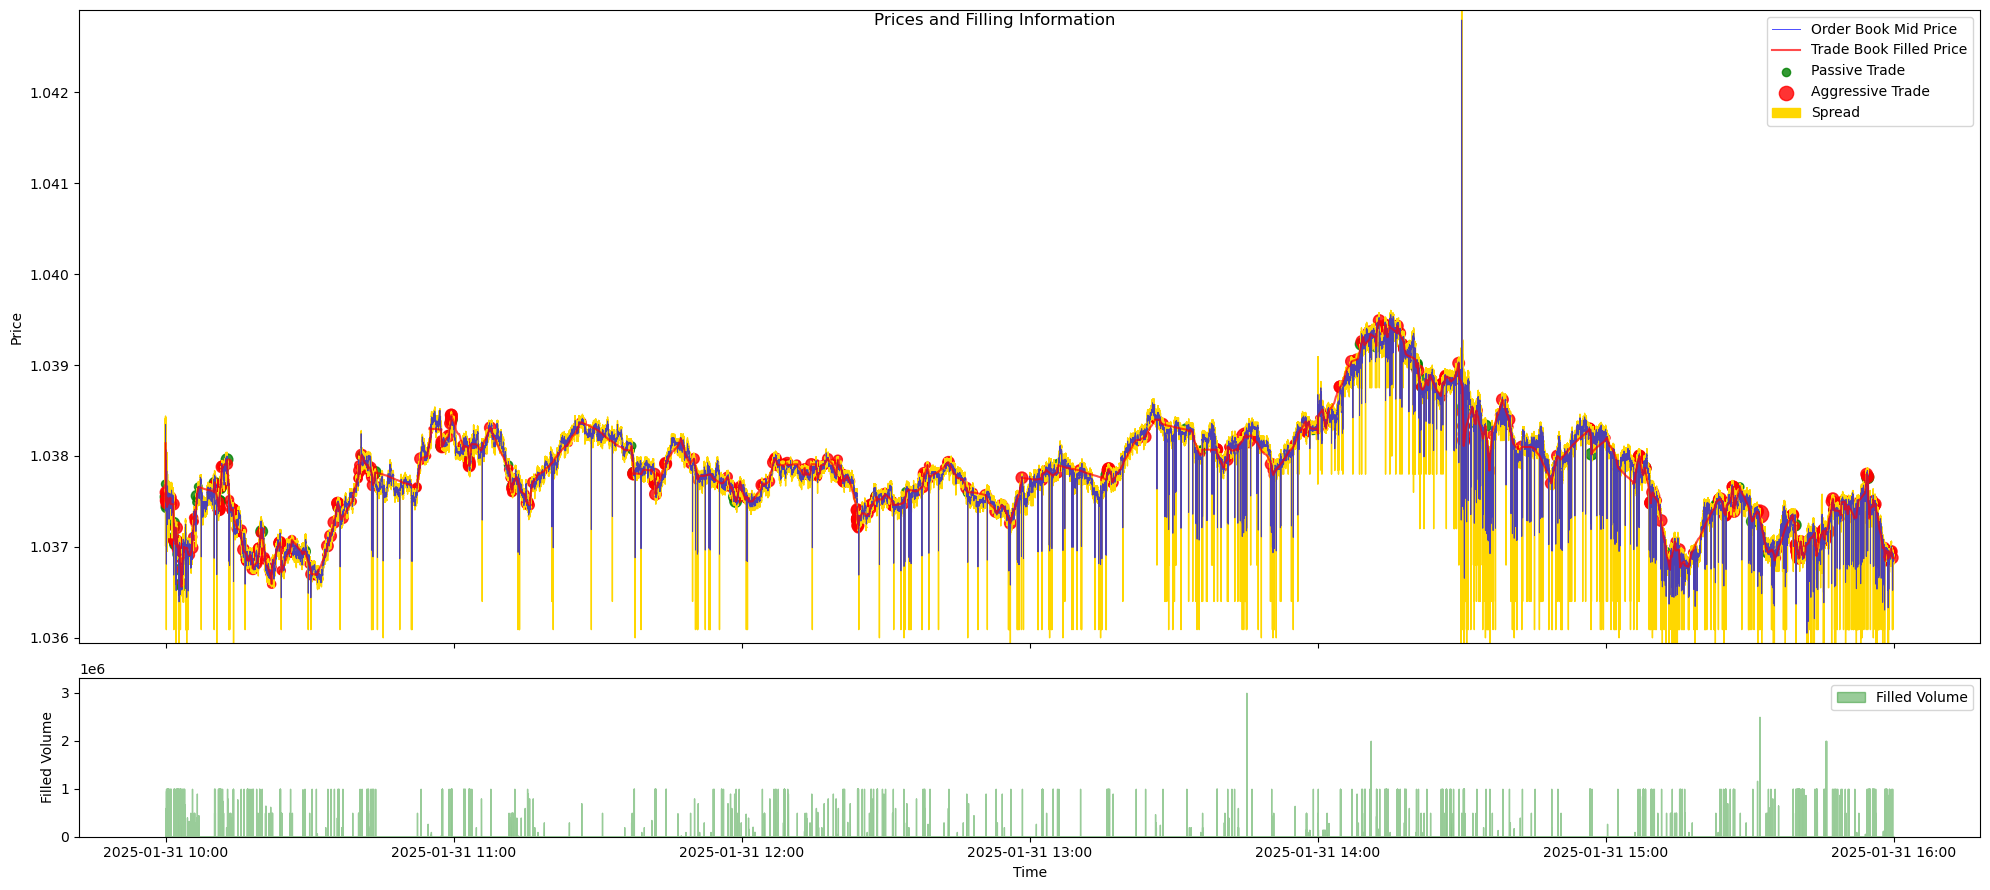
\includegraphics[width=1\linewidth]{figures/Prices and Filling Information.png}
    \caption{Prices and filling information. This plot shows the mid-price from the order book (blue line), trade book filled prices (red line), and spread (yellow shading). Passive trades (green dots) and aggressive trades (red dots) are highlighted. The bottom panel represents the filled volume over time.}
    \label{fig:p_f_i}
\end{figure}
As can be seen in Figure~\ref{fig:p_f_i}, the mid-price has the highest point between 14:00 and 15:00. The filled price fits the mid-price well. We can see there are a lot of red dots which shows that they are aggressive trades. We didn't classify bid or ask side because it's not the research target in the thesis. These aggressive trades go outside the spread range. The size of dots stands for relative volume of the trades. In other words, when the volume is large compared to other timestamps, the size of the dot will be larger. Therefore, we can easily see the active trading time point in the plot. Moreover, red dots represent aggressive trades in the trade book. We can see the red dots are more than green ones, which indicates that a lot of orders get filled by aggressive traders taking out them of the order book, instead of passively waiting for the market movements. This aligns with our need to improve the backtesting environment by predicting aggressive trades across the order book. Specially, there are several sparks in the trend of mid-price in the order book. These are caused by...

From the bottom panel, in the beginning of 10:00, 15:45, 14:11, there are high volume up to 2,000,000, which are higher than common volume 1,000,000. At 13:45, the highest trading volume occurs as 3,000,000. Combined the two plots together, we can see when there's a drop, it's often accompanied by many trading records or large trades. 

\begin{figure}[h]
    \centering
    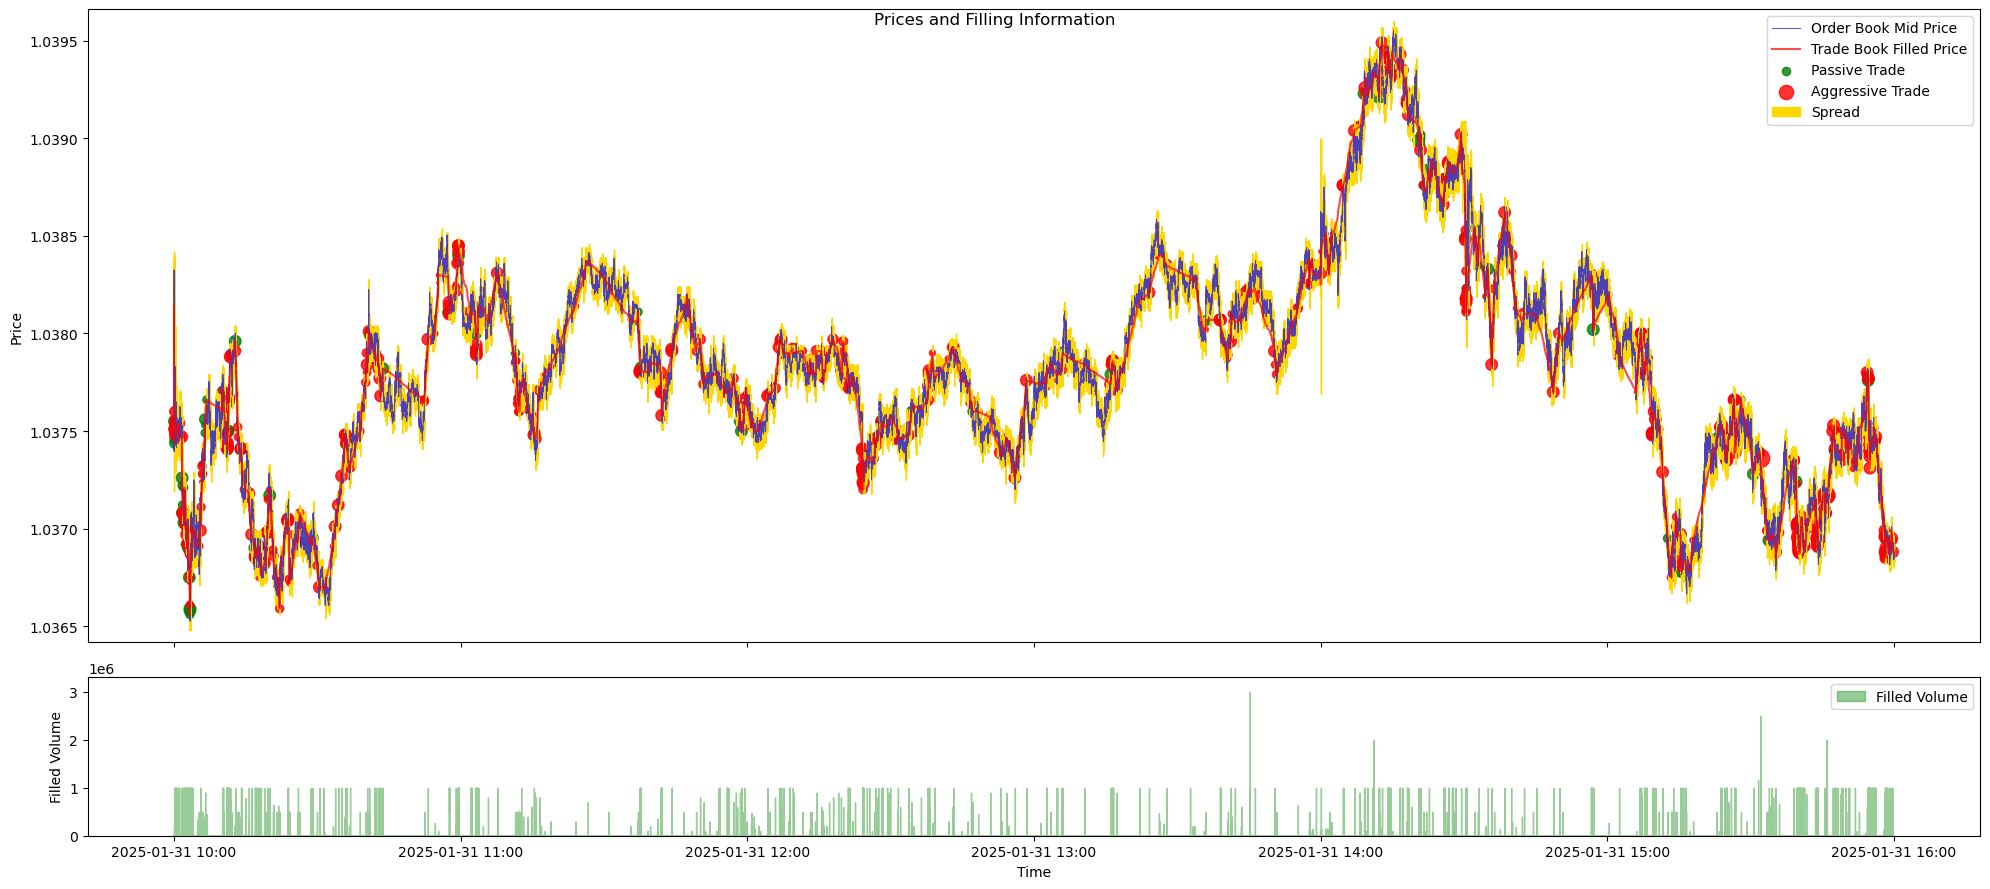
\includegraphics[width=1\linewidth]{figures/Filtered Prices and Filling Information.png}
    \caption{Filtered prices and filling information. Similar to Figure~\ref{fig:p_f_i}, but filtering sharp jump points. The price and trade dynamics remain the same, without increased variability for better general trend capture}
    \label{fig:f_p_f_i}
\end{figure}

In the Figure~\ref{fig:f_p_f_i} after filtering 1,232 sparks in the data, we can clearly see some clustering for both passive and aggressive trades. For example, in the beginning of 10:00, many passive trades gather here. It may because there's a sharp dropping movement in the market, many limit orders are filled. Furthermore, many aggressive trades gather around  


% Evaluating how well the model captures aggressive trades movements and distribution.
% Market realism (stylized facts: price impact, spread, volume clustering).
\section{Step-by-Step Prediction Results}
The prediction framework consists of three sequential stages. The first stage employs an XGBoost model to identify potential aggressive trade timestamps while reducing the overall dataset size. The second stage is GRU networks. It serves as a bridge between machine learning approaches and stochastic processes, centering around potential timestamps where trades could happen from XGBoost to improve the class balance and generate high-confidence timestamps likely to contain aggressive trades. The final stage implements a tailored Hawkes process that estimates event intensity while incorporating MN's specific trading information. In the end this multi-stage approach produces a detailed and interpretable set of predictions for potential aggressive trading events.

We present the prediction results of each stage using a representative trading day. The training dataset consists of the whole trading day from January 31, 2025, 10:00:00 to 15:59:59 PM, containing 307,764 rows. The testing dataset is a 30-minute window from January 30, 2025, 09:08:57 to 09:38:51, with 18,848 rows. This specific time window was selected as it represents a commonly used timeframe for FX trading backtesting within the MN platform.

\subsection{XGBoost Stage: With and Without KMeansSMOTE}
KMeansSMOTE, introduced in the Methodology chapter, is an oversampling technique designed to address class imbalance in training data. We compare the XGBoost prediction results with and without KMeansSMOTE to evaluate the influence of oversampling. The impact of applying this oversampling method on both class balance and prediction quality is analyzed.

We first present the classification results of XGBoost trained with KMeansSMOTE. The KMeansSMOTE configuration is as follows:

\begin{verbatim}
pipeline = Pipeline([
("imputer", SimpleImputer(strategy="median")),
("smote", KMeansSMOTE(random_state=42,
cluster_balance_threshold=0.002,
kmeans_estimator=KMeans(n_clusters=200, random_state=42),
sampling_strategy=0.5))
])
\end{verbatim}

The median strategy fills missing values with the median of each feature. A cluster balance threshold of 0.02 ensures oversampling is done in 'safe' areas where there are at least some genuine minority examples. This can improve sample quality and reducing class overlap or overfitting risks. As a result, the training set has equal amounts of class 1 and class 0, but most class 1 samples are artificially created by oversampling.

%from here start
As shown in Figure~\ref{fig:xgb-pred-vs-true-km}, the model catches many true positives. The class balancing done by KMeansSMOTE reduces the bias toward class 0 and helps the model learn better from the underrepresented class 1.

Table~\ref{tab:xgb-confusion-km} shows the confusion matrix. There are 11,545 test samples after filtering. Among them, 11,487 are predicted as class 0 (no trade), and only 58 are predicted as class 1 (trade). The model correctly finds 39 true positives and 7,293 true negatives. The dataset size drops from 18,848 to 11,545 rows, which is 38.75\% of the original. This helps improve speed and keeps most of the important trade points.

Moreover, Table~\ref{tab:xgb-classification-report-km} shows the detailed classification report. We mainly care about the prediction performance for class 1, since this is the main goal of the whole research. The precision of class 0 is not meaningful here because the original data is extremely imbalanced. Although the precision for class 1 is still very low at 0.0034, the recall reaches 0.5735. This means the model finds more true trades, even though oversampling brings some noise. This makes preparation for next GRU networks to train around aggressive trades timestamps. The F1-score for class 1 is 0.0067, but this result already gives a good starting point for the next filtering stages.


\begin{figure}[H]
    \centering
    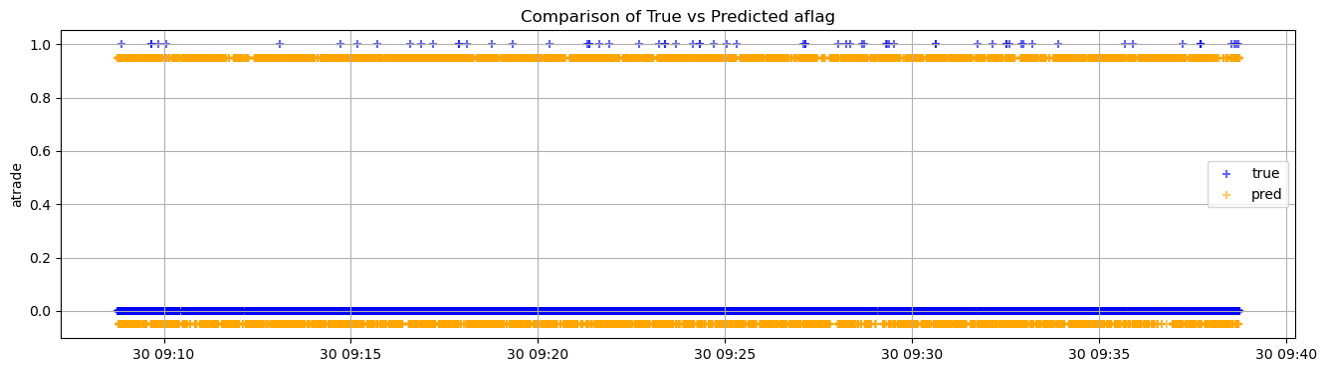
\includegraphics[width=\textwidth]{figures/XGBoost comparison1.png}
    \caption{Comparison of true vs. predicted $\bar{\alpha}$ from XGBoost with KMeansSMOTE. 
    The blue '+' markers show the true class labels, and the orange '+' markers show the predicted ones. To make the plot easier to read, the predicted values are moved down by 0.05 on the y-axis. This small shift helps to see clearly how well the predictions match the true labels.
    }
    \label{fig:xgb-pred-vs-true-km}
\end{figure}

\begin{table}[H]
    \centering
    \caption{Confusion matrix of XGBoost with KMeansSMOTE}
    \label{tab:xgb-confusion-km}
    \begin{tabular}{lcc}
        \toprule
        & Predicted 0 & Predicted 1 \\
        \midrule
        True 0 & 7,293 & 11,487 \\
        True 1 & 29 & 39 \\
        \bottomrule
    \end{tabular}
\end{table}
\begin{table}[H]
    \centering
    \caption{Classification report of XGBoost with KMeansSMOTE}
    \label{tab:xgb-classification-report-km}
    \begin{tabular}{lcccc}
        \toprule
        Class & Precision & Recall & F1-score & Support \\
        \midrule
        0 & 0.9962 & 0.3882 & 0.5587 & 18780 \\
        1 & 0.0035 & 0.5882 & 0.0069 & 68 \\
        \midrule
        Accuracy & \multicolumn{4}{c}{0.3890} \\
        Macro avg & 0.4998 & 0.4882 & 0.2828 & 18848 \\
        Weighted avg & 0.9926 & 0.3889 & 0.5567 & 18848 \\
        \bottomrule
    \end{tabular}
\end{table}

Without KMeansSMOTE, even if we reach the same recall, the precision is even worse (only 0.0019). That means almost all predicted class 1 are wrong. The F1-score is just 0.0038, which is only half of the score from XGBoost with KMeansSMOTE. Also, the filter effect is weaker. More lines (12,479) are left in the result, which makes the next detection step slower and more difficult. So using KMeansSMOTE helps not only improve model performance but also makes the pipeline more efficient.

\begin{table}[H]
    \centering
    \caption{Confusion matrix of XGBoost without KMeansSMOTE}
    \label{tab:xgb-noKM}
    \begin{tabular}{lccc}
        \toprule
        Class & Precision & Recall & F1-score\\
        \midrule
        1 & 0.0019 & 0.5881 & 0.0038 \\        
        \bottomrule
    \end{tabular}
\end{table}

These results show that KMeansSMOTE gives significant improvement when dealing with extreme class imbalance, especially in terms of F1-score. The large set of candidate points predicted at this stage will be passed to the next GRU model, which helps to further clean and refine the aggressive trade signals.

\subsection{GRU Stage: With and Without Window-Based Filtering}
The GRU model is used to make up for XGBoost's weakness in learning the order of data. XGBoost gives high recall and selects good features, but it looks at each sample alone and cannot understand the sequence in order book data. GRU, as a recurrent neural network, is better for learning patterns over time.

We compare the GRU model trained on window-filtered data and unfiltered data. The window-based filtering puts the focus around class 1 events, which helps improve signal quality and class balance. The test data is the output from XGBoost.

The GRU model is trained on window-filtered data. As shown in Figure~\ref{fig:win-gru-distribution}, the class balance improves a lot. Class 1 now takes up 18.7\% of the training data. Before applying this filter, class 1 was only 0.2\%, as shown in Figure~\ref{fig:aflag_class_distribution}. So this step really helps the model learn the aggressive trade pattern better. 

The test data comes from the output of KM-XGBoost. This makes the test set match the features of the training data of GRU. After this GRU stage, the total number of samples becomes 7307, which is much smaller than before and lightweight enough for running the Hawkes process in the final stage. So this step helps not only with learning quality but also with efficiency.

In Figure~\ref{fig:win-gru-pred-vs-true}, we compare the predictions with the true labels. The blue '+' markers are the true values, and the orange '+' markers are the predicted ones. As before, the predicted values are shifted down by 0.05 on the y-axis to make the comparison easier. We can see that the orange points now align more closely with the blue ones, especially in the class 1 area. So the GRU model starts to catch aggressive trades more accurately.

The confusion matrix and classification report are shown in Table~\ref{tab:win-gru-metrics}. The recall for class 1 is 0.4792, which is not perfect but already acceptable. The precision is 0.0146, but better than in the XGBoost stage. The F1-score is 0.0283, which means this GRU step helps to clean the signal after the broad filtering done by XGBoost. The output dataset is then sent to the Hawkes process for simulation.

\begin{figure}[H]
    \centering
    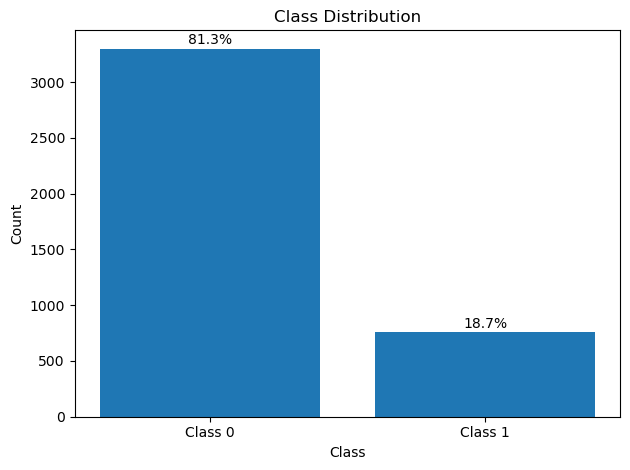
\includegraphics[width=0.5\textwidth]{figures/win_gru_distribution.png}
    \caption{Class distribution after applying window-based filtering in GRU training data. Class 1 increases from 0.02\% to 18.7\%.}
    \label{fig:win-gru-distribution}
\end{figure}

\begin{figure}[H]
    \centering
    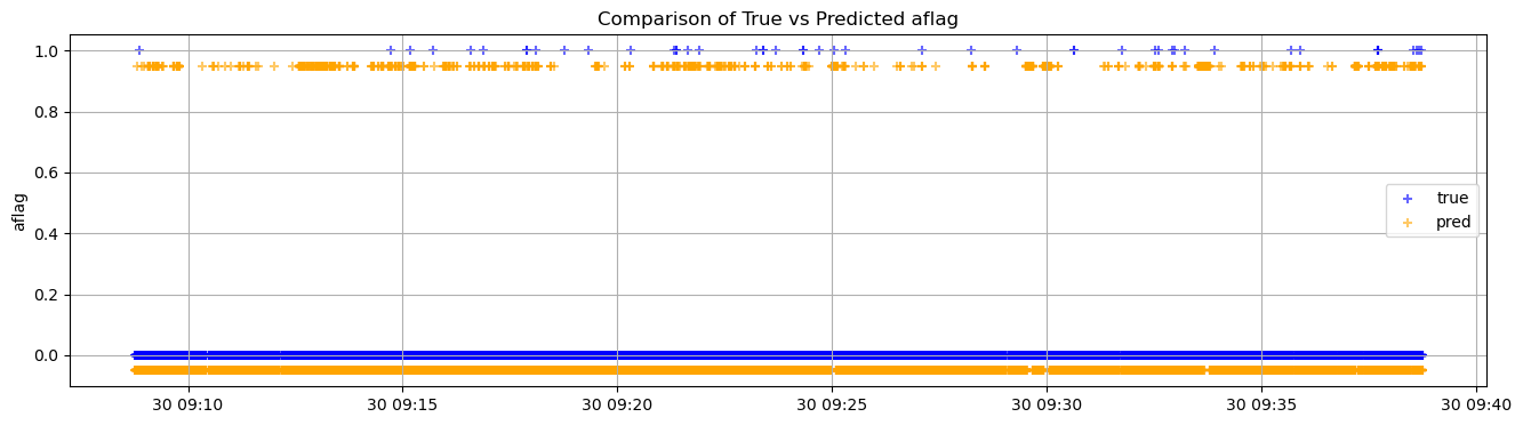
\includegraphics[width=\textwidth]{figures/win_gru_pred_vs_true.png}
    \caption{Window-based GRU: comparison of predicted and true $\bar{\alpha}$. Prediction shifted -0.5 for visibility.}
    \label{fig:win-gru-pred-vs-true}
\end{figure}

\begin{table}[H]
    \centering
    \caption{Confusion matrix and classification report of window-based GRU}
    \label{tab:win-gru-metrics}
    \begin{tabular}{lccc}
        \toprule
        Class & Precision & Recall & F1-score\\
        \midrule
        1 & 0.0146 & 0.4792 & 0.0283 \\
        \midrule
        \textbf{Confusion Matrix} & \multicolumn{3}{c}{} \\
        \midrule
        & Pred 0 & Pred 1 &  \\
        \midrule
        True 0 & 17246 & 1554 &  \\
        True 1 & 25 & 23 &  \\
        \bottomrule
    \end{tabular}
\end{table}

\newpage

\subsection{Hawkes Stage: Feasibility and Efficiency}
%need to do more explaination to show how the result is interpreable
Directly applying the Hawkes process to the full dataset is very slow. It takes more than 12 hours to run, which is not realistic in trading environments. So here, we only use the filtered test timestamps from the WinGRU stage to do simulation, and estimate the Hawkes parameters based on the KM-XGBoost output, which has high recall. This makes the simulation much faster and also cleaner because we already removed lots of noise in previous steps.

In Figure~\ref{fig:hawkes-simulation}, we can see that the simulated event type distribution and timeline match the original ones quite well. The model keeps the overall shape of trading activity, and the inter-arrival time distribution is also similar between real and simulated. So the simulation is doing a good job in capturing the market flow.

Figure~\ref{fig:hawkes-pred-vs-true} shows the predicted versus true aggressive trades. Again, blue '+' are the ground truth, and orange '+' are predicted, shifted down a bit for easier comparison. The pattern is sparser than WinGRU, but still keeps many correct signals.

Table~\ref{tab:hawkes-metrics} gives the classification result. Now the precision reaches 0.2, which is much better than before. The recall is 0.1667, and F1-score is 0.1818. This shows Hawkes simulation is more conservative, but the predictions it gives are more accurate. So this final stage helps us get high-quality aggressive trade points for analysis or action.

Table~\ref{tab:hawkes-metrics} shows the classification result. Now the precision reaches 0.2, which is much better than before. The recall is 0.1667, and the F1-score is 0.1818. This shows that the Hawkes simulation is more conservative, but the predictions it gives are more accurate. So this final stage helps us get high-quality aggressive trade points which is more reasonable to be applied to FX trading backtesting.

\begin{figure}[H]
    \centering
    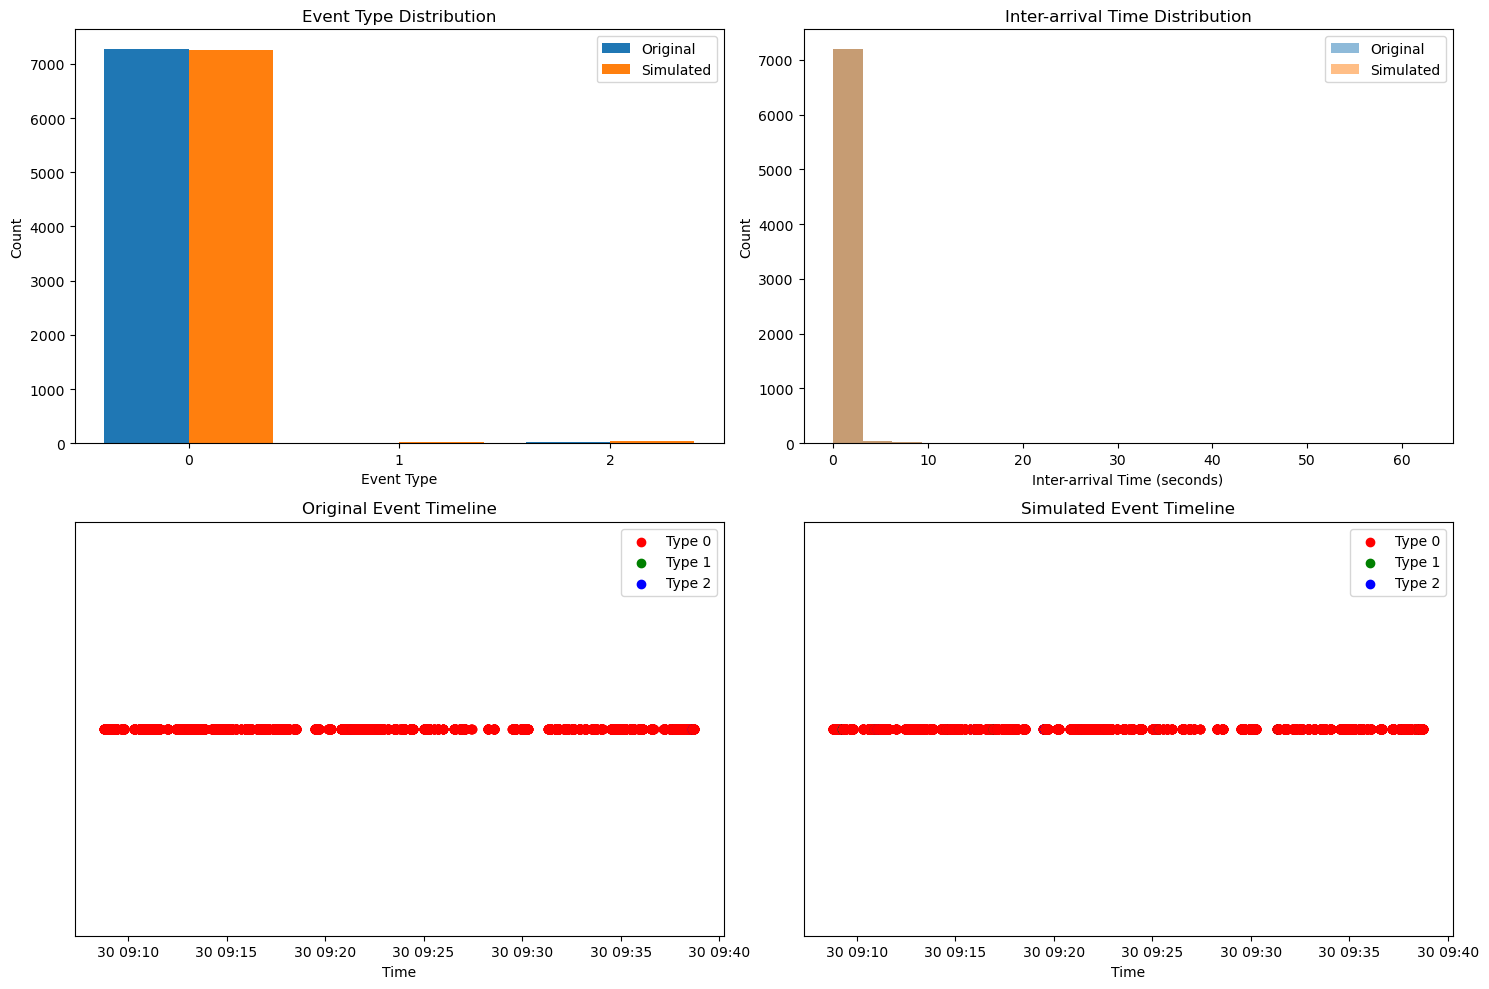
\includegraphics[width=\textwidth]{figures/hawkes_simulation.png}
    \caption{Hawkes process simulation result: event type distribution, inter-arrival time, and timeline comparison.}
    \label{fig:hawkes-simulation}
\end{figure}

\begin{figure}[H]
    \centering
    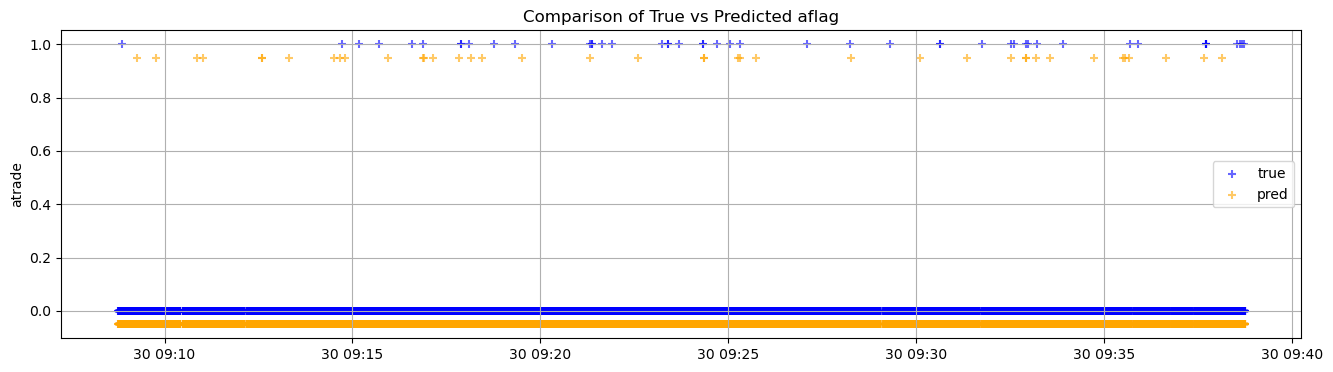
\includegraphics[width=\textwidth]{figures/hawkes_pred_vs_true.png}
    \caption{Comparison of true vs. predicted $\bar{\alpha}$ from Hawkes simulation. Prediction is shifted -0.5 on the y-axis.}
    \label{fig:hawkes-pred-vs-true}
\end{figure}

\begin{table}[H]
    \centering
    \caption{Confusion matrix and classification report of Hawkes simulation}
    \label{tab:hawkes-metrics}
    \begin{tabular}{lccc}
        \toprule
        Class & Precision & Recall & F1-score \\
        \midrule
        1 & 0.2000 & 0.1667 & 0.1818 \\
        \midrule
        \textbf{Confusion Matrix} & \multicolumn{3}{c}{} \\
        \midrule
        & Pred 0 & Pred 1 & \\
        \midrule
        True 0 & 18768 & 32 & \\
        True 1 & 40 & 8 & \\
        \bottomrule
    \end{tabular}
\end{table}

\subsection{Result Conclusion and Data Flow}
\begin{figure}[H]
    \centering
    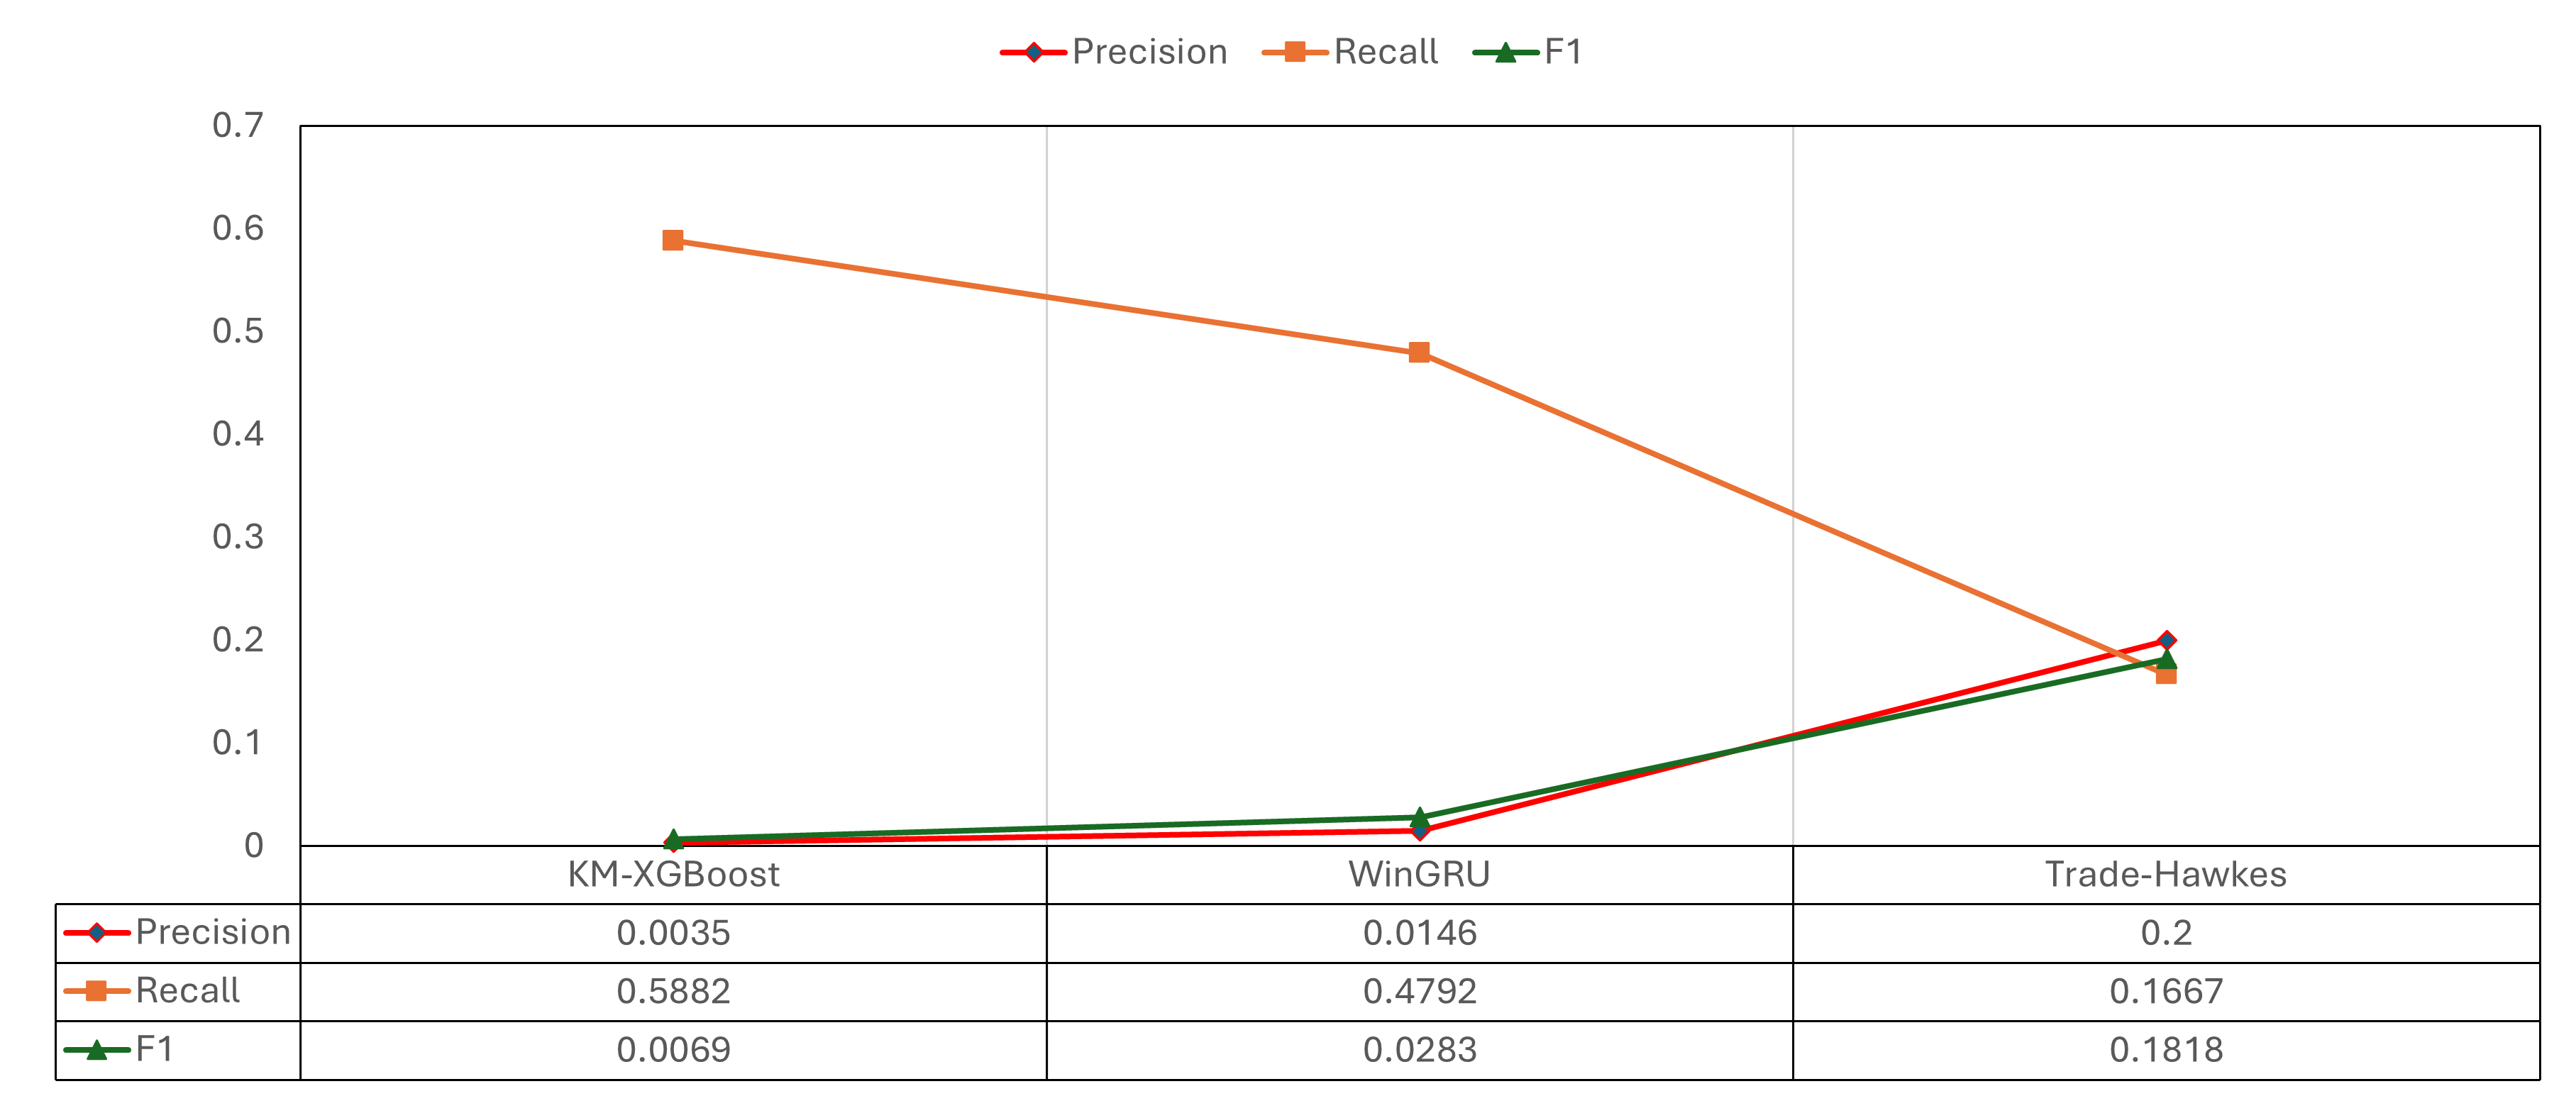
\includegraphics[width=0.9\textwidth]{figures/final_performance_plot.png}
    \caption{Precision, recall, and F1-score across different stages.}
    \label{fig:final-performance}
\end{figure}

\begin{figure}[H]
    \centering
    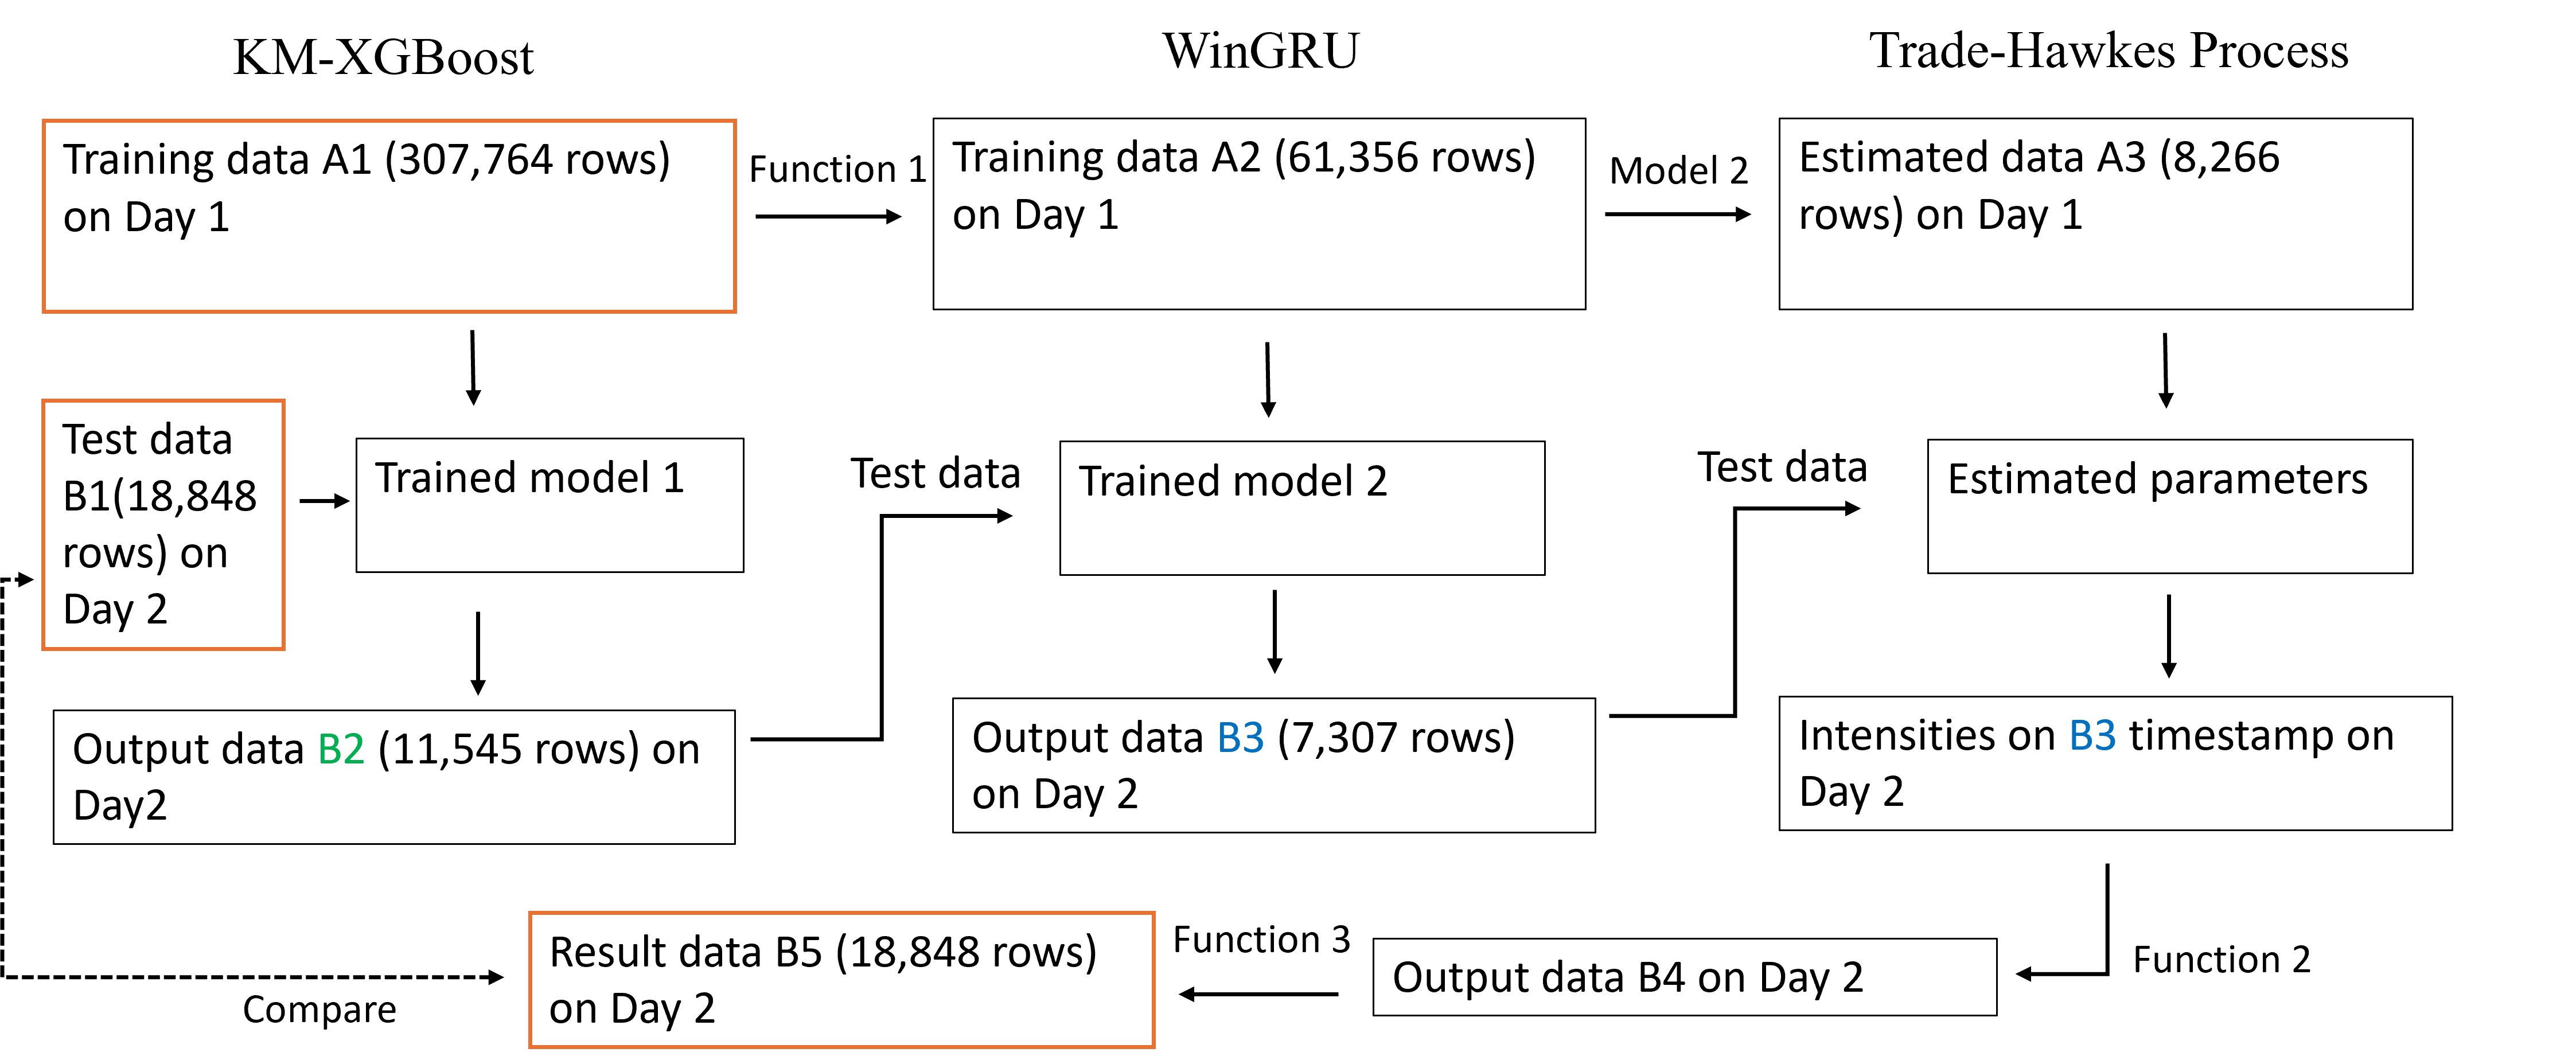
\includegraphics[width=\textwidth]{figures/data flow.png}
    \caption{Data flow of the full pipeline from raw data to final prediction.}
    \label{fig:data-flow-diagram}
\end{figure}

\section{Overall Framework Results}
In this section, we evaluate the performance of the Two-stage Machine Learning and Stochastic Modeling Framework on different trading days, including. The results are compared against several single-model benchmark models, such as only XGBoost, only GRU and Hawkes process. This comparison demonstrates the accuracy and effectiveness of the combined framework in improving simulation performance, particularly under extreme class imbalance.













% \section{Prediction for $\bar{\alpha}$}
% \begin{figure}[h]
%     \centering
%     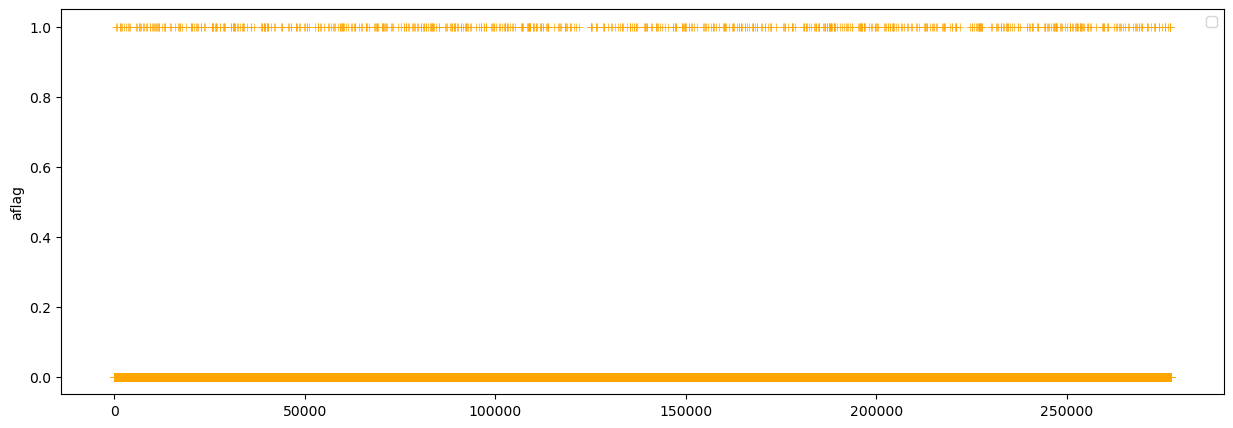
\includegraphics[width=\linewidth]{figures/aflag.png}
%     \caption{Binary distribution of the aggressive trade flag $\bar{\alpha}$}
%     \label{fig: aflag}
%     {\small \textit{Note.} Each point with value 1 indicates the occurrence of an aggressive trade, while 0 indicates non-aggressive or no trade.}
% \end{figure}
% Figure.~\ref{fig: aflag_class_distribution} shows $\bar{\alpha}$ faces severe class imbalance, which can lead to biased model predictions if not addressed. Class 0 dominates the dataset, accounting for 99.8\% of all samples, while Class 1 accounts for only 0.2\%. To solve this imbalance, techniques such as resampling, weighted loss functions, and anomaly detection methods are employed. 
% \begin{figure}[h]
%     \centering
%     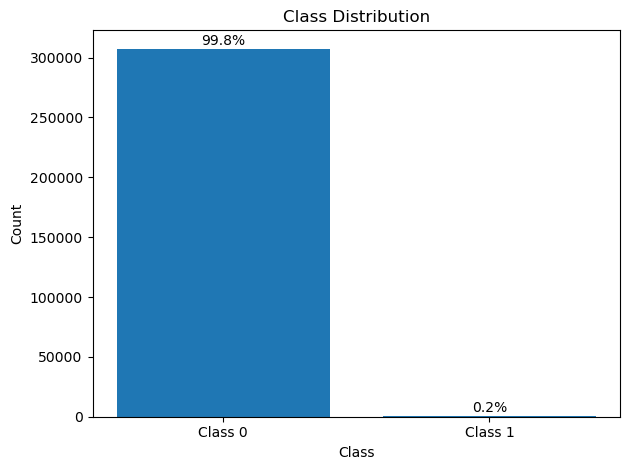
\includegraphics[width=0.8\linewidth]{figures/Imbalaced data for aflag.png}
%     \caption{Class Distribution for $\bar{\alpha}$}
%     {\small \textit{Note.} In the overall 308,178 data, class 0 accounts for 99.8\% of the samples, while Class 1 represents only 0.2\%, indicating a severe class imbalance.}
%     \label{fig: aflag_class_distribution}
% \end{figure}
% \newpage
% \subsection{XGBoost}
% \begin{figure}[h]
%     \centering
%     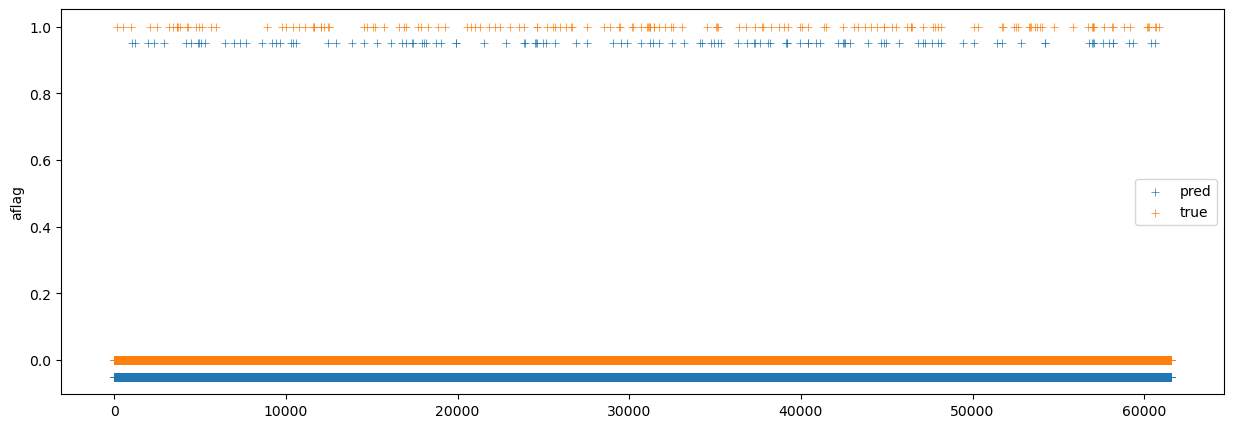
\includegraphics[width=\linewidth]{figures/aflag_XGBoost.png}
%     \caption{Predicted and true values of $\bar{\alpha}$}
%     \label{fig:aggressive_flag_prediction}
%     {\small \textit{Note.} The plot compares the predicted and true values of the aggressive flag. Each `+` marker represents a positive prediction (blue) or ground truth (orange). The strong class imbalance and sparsity of positive cases make correct prediction more difficult, highlighting the challenge of this classification task.}
% \end{figure}
% The model's performance on the test set is summarized by the confusion matrix and associated classification metrics. 

% \begin{table}[h]
% \centering
% \caption{Confusion Matrix}
% \begin{tabular}{c|cc}
% \toprule
%               & Predicted 0 & Predicted 1 \\
% \midrule
% Actual 0      & 61311       & 99          \\
% Actual 1      & 136         & 17          \\
% \bottomrule
% \end{tabular}
% \label{tab:confusion_matrix}
% \vspace{2mm}

% {\small \textit{Note.} The confusion matrix shows a strong true negative rate but a weak true positive rate, which is expected in highly imbalanced classification tasks.}
% \end{table}

% \begin{table}[h]
% \centering
% \caption{Classification Report}
% \begin{tabular}{lcccc}
% \toprule
% Class & Precision & Recall & F1-score & Support \\
% \midrule
% 0     & 0.9978    & 0.9984 & 0.9981   & 61410   \\
% 1     & 0.1466    & 0.1111 & 0.1264   & 153     \\
% \midrule
% Accuracy     & \multicolumn{3}{c}{0.9962} & 61563 \\
% Macro Avg    & 0.5722 & 0.5547 & 0.5622   & 61563 \\
% Weighted Avg & 0.9957 & 0.9962 & 0.9959   & 61563 \\
% \bottomrule
% \end{tabular}
% \label{tab:classification_report}
% \vspace{2mm}

% {\small \textit{Note.} While the overall accuracy is high due to the dominance of class 0, the metrics for class 1 reveal the difficulty of detecting aggressive trades.}
% \end{table}

% \noindent
% \textbf{AUC:} 0.6424
% {\small \textit{Note.} The Area Under the Curve (AUC) score indicates the ability to separate the two classes.}

% \subsection{Feature Importance}
% \begin{figure}[h]
%     \centering
%     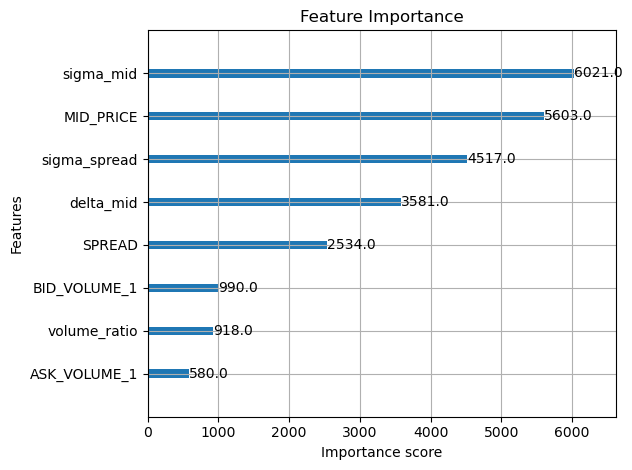
\includegraphics[width=\linewidth]{figures/feature importance.png}
%     \caption{Feature importance scores for predicting aggressive trades}
%     \label{fig:feature_importance_af}
%     {\small \textit{Note.} The most important features include \texttt{sigma\_mid}, \texttt{MID\_PRICE}, and \texttt{sigma\_spread}, indicating that mid-price volatility and spread dynamics play a key role in identifying aggressive trade behavior. Volume-related features such as \texttt{ASK\_VOLUME\_1} and \texttt{BID\_VOLUME\_1} are less influential.}
% \end{figure}

% \newpage


% \section{Prediction for $\alpha$}
% \begin{figure}[h]
%     \centering
%     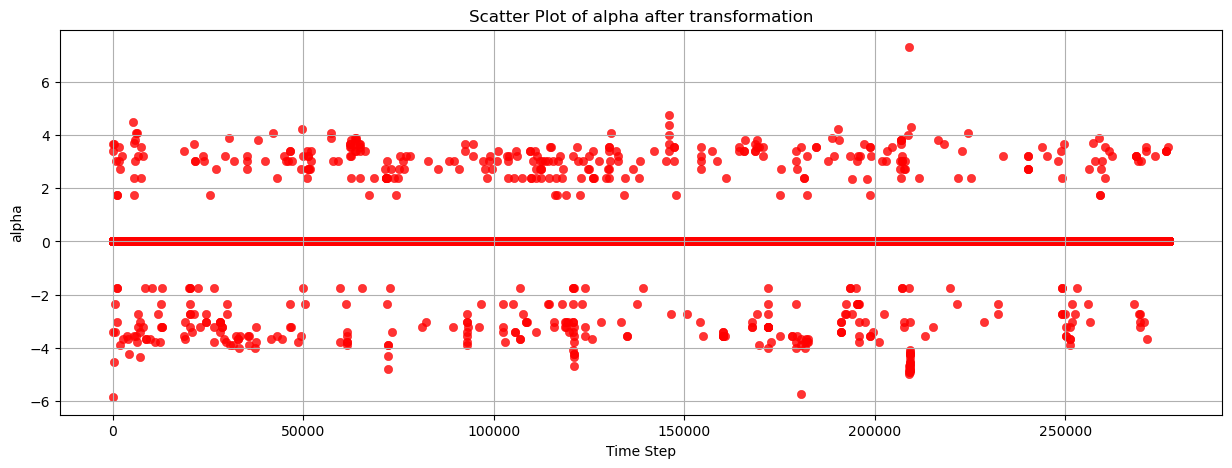
\includegraphics[width=\linewidth]{figures/alpha after transformation.png}
%     \caption{Scatter plot of transformed $\alpha$ values over time}
%     \label{fig:alpha_transformed_scatter}
%     {\small \textit{Note.} This plot visualizes the transformed $\alpha$ signal across time steps. Most values are concentrated near zero, while some are clearly positive or negative.}
% \end{figure}
% \subsection{GRU-based Neural Network}
% \begin{figure}[h]
%     \centering
%     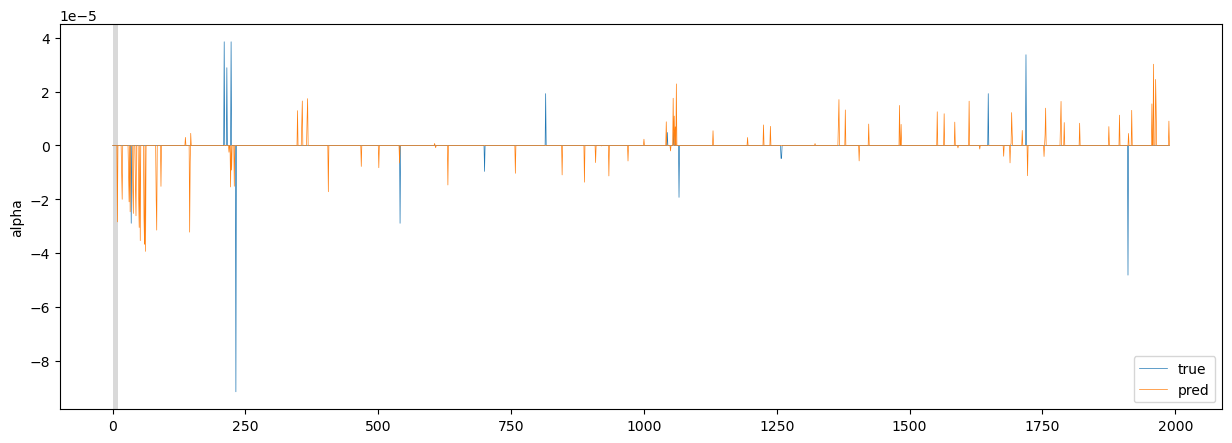
\includegraphics[width=\linewidth]{figures/alpha_GRU.png}
%     \caption{Prediction of $\alpha$ using a GRU-based model}
%     \label{fig:gru_alpha_prediction}
%     {\small \textit{Note.} This plot compares the predicted $\alpha$ values from a GRU model (orange) against the ground truth (blue). The GRU captures some local patterns.}
% \end{figure}
% \begin{figure}[h]
%     \centering
%     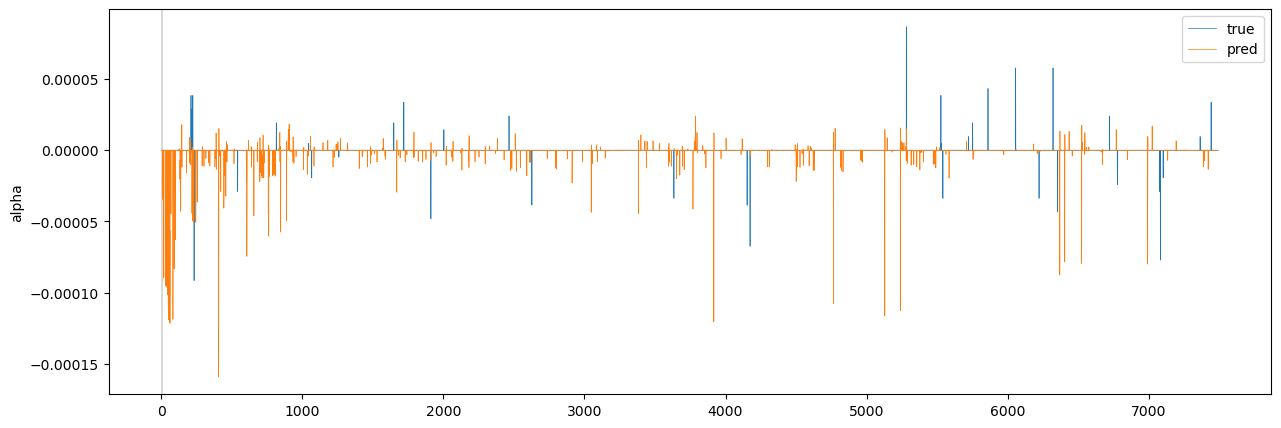
\includegraphics[width=\linewidth]{figures/alpha_Linear.png}
%     \caption{Prediction of $\alpha$ using a linear regression model}
%     \label{fig:lr_alpha_prediction}
%     {\small \textit{Note.} The linear regression model shows limited ability to capture fluctuations in $\alpha$, often underestimating both amplitude and timing compared to the true values. This highlights the limitations of linear models in capturing non-linear temporal dependencies.}
% \end{figure}

% \begin{table}[h]
%     \centering
%     \caption{Performance comparison between GRU and Linear Regression for $\alpha$ prediction}
%     \label{tab:gru_vs_lr}
%     \begin{tabular}{lcc}
%         \toprule
%         Metric & GRU & Linear Regression \\
%         \midrule
%         MSE   & 0.1348  & 0.3336 \\
%         RMSE  & 0.3672  & 0.5776 \\
%         MAE   & 0.0263  & 0.0367 \\
%         %R$^2$ & 3.1362  & 21.0387 \\
%         MAPE (\%) & 63.47  & 62.74 \\
%         SMAPE (\%) & 59.95  & 62.11 \\
%         \bottomrule
%     \end{tabular}
% \end{table}
% Table~\ref{tab:gru_vs_lr} compares the performance of the GRU model and the linear regression model on the task of predicting $\alpha$. The GRU model achieves lower MSE (0.1348 vs. 0.3336), RMSE (0.3672 vs. 0.5776), and MAE (0.0263 vs. 0.0367), indicating better overall prediction accuracy. Although both models show similar MAPE and SMAPE values, the GRU produces a slightly lower symmetric error. 
% % The R$^2$ values are unusually high for both models, likely due to the small magnitude of $\alpha$ and possible data scaling effects, but the relative comparison still shows the GRU outperforming the linear model. 
% Overall, the GRU model demonstrates better capability in capturing the temporal and nonlinear dynamics of the data.

% \section{Prediction for $\tau$}
% Figure.~\ref{fig: Countdown} shows how much time is left until the next aggressive trade. Each point at 0 represents for an aggressive trade. After each zero point, a sharp increase marks the start of a new countdown period leading up to the next aggressive trade.
% \begin{figure}[h]
%     \centering
%     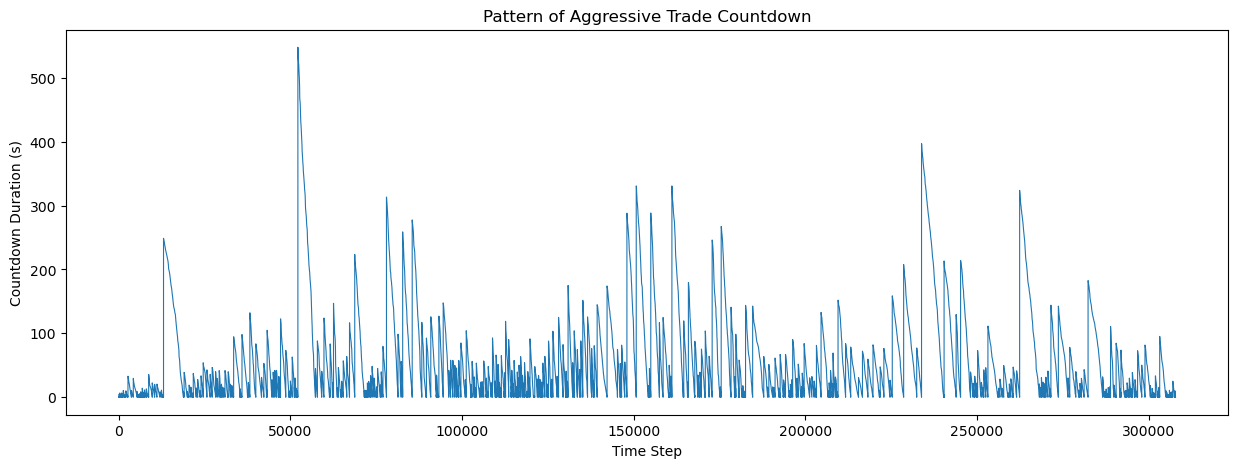
\includegraphics[width=\linewidth]{figures/Pattern of Aggressive Trade Countdown.png}
%     \caption{Countdown to the next aggressive trade}
%     \label{fig: Countdown}
% \end{figure}

% \subsection{XGBoost}
% \subsection{Recurrent Neural Networks}
% The feature matrix $X$ and the target vector $y$ are converted to NumPy arrays. The dataset is split into training (90\%) and testing (10\%) sets. Both the input and output are scaled to improve convergence during training. Inputs are normalized to the range $[0, 1]$ using a MinMaxScaler. For the output, to enhance the sensitivity of the model to small but informative signals, we applied a signed logarithmic transformation to selected features. The transformation preserves the original sign of the data, compresses large magnitudes, and expands small nonzero values, making subtle patterns more noticeable to the model. After applying the logarithmic adjustment, the transformed values are rescaled to fit within the range \([-1, 1]\). An inverse transformation is also defined to recover the original values when necessary, maintaining consistency between the transformed and original feature spaces.


% \section{Ablation Studies}
% Impact of different model components (CGAN vs. pure Hawkes vs. hybrid). Sensitivity analysis on model hyperparameters.


% \section{Backtesting Performance}
% Simulating market impact with aggressive/passive execution strategies.
% Evaluating execution cost and slippage in various market scenarios.
% Comparing execution performance with traditional historical replay.

% \section{Application to other products}
% other products, like FX options, equity...

\chapter{Conclusion and Future Recommendations}\label{chapter:cd}
% discussion of the outcomes
In conclusion, the results in Chapter~\ref{chapter:experiments} show that our framework has good alignment with real FX spot market in both the market conditions, temporal dependencies and clustering properties of aggressive trades. By using the XGBoost filter, class imbalance gets solved, and the Neural Hawkes Process is able to fits well with the true pattern of aggressive trade. The model gives realistic and dynamic predictions, which are two critical requirements confirmed by evaluation metrics results. By clear short-term excitation, fast decay, and intensity, the model is capable to be explained clearly why an aggressive trade occurs and why not. It is more robust and transparent than black-box models, and more sophisticated and dynamic than single stochastic model. It is useful for building better and more realistic backtesting environments.

% Comparison with Existing Approache, simplications for FX backtesting environments
Compared to the existing backtesting approach at MN as shown in Table~\ref{tab:filling_spread}, our method gives a more realistic and dynamic view of order filling method. The traditional backtesting method uses filling probabilities based on spread only. This is simple and fast, but it does not reflect how aggressive trades happen in the market, thus loses many transaction opportunities. It ignores the clustering of trades and changes in market conditions. By the use of our model, it captures how often trades happen and when they happen. This makes the backtesting more realistic, dynamic and closer to real market scenarios. 

% Potential applications beyond FX, e.g., equities, crypto markets.
Besides the use in FX spot market, it is also appliable in other high-frequent trading markets, like equities and crypto. Outside the financial field, it can also be used for classification prediction problems with extreme class imbalance, like medical disease detection, fraud detection in banking, network intrusion detection in cybersecurity, and rare event prediction in industrial systems. In all these cases, events are rare, depend on time and conditions, and require models that can capture both sequence and intensity patterns, which our framework is designed to do.

% Future Research Directions and possible improvement
There are also some ways to improve our work in the future. First, the model can be extended to simulate multiple types of market events, not just aggressive trades. This would help build a more complete market environment. Second, the current model focuses on one market. Future work can explore multi-asset or cross-market scenarios to test trading strategies across different markets. Finally, the model now uses fixed features calculated by order book information for prediction. It might help to include more features, such as news sentiment. 

\printglossary[type=\acronymtype, title=Acronyms]
\printglossary

%Choose a good bibliography style, plain would do often, but these might be nice too
%\bibliographystyle{these}
\bibliography{references}

\newpage
\appendix
\input{appendices/main}


\end{document}
